\chapter{Evaluation and Analysis}
\label{chapter:evaluationAnalysis}

In the previous chapter, we present a few approaches that could improve the genetic solver.
The best results give the \textbf{NP} version of the genetic solver. It is a combination of the genetic solver with added probabilities and parameter tuning.
Other methods like a crossover rate with parameter control or population without duplicated individuals have less effect on the results.

However, we get valid results only for one problem. But what if we change the complexity of the problem? We perform the benchmark to find out how all approaches work with different problem sizes. 

\section{Evaluation}
\label{sec:evaluation}

To evaluate the genetic solver, we perform a set of benchmarks that consist of 36 problems~(see Appendix~\ref{appendix:ProblemSet}). Each problem has different parameters that describe~(Section~\ref{sec:MQuATProblem}) it:

\begin{itemize}
	\item Software variants: [2, 4];
	\item Number of requests: [1, 2, 4];
	\item Component tree depth: [2, 3, 4];
	\item Resources ratio: [50, 100].
\end{itemize}

This set of problems is tested with several versions of the genetic solver:

\begin{itemize}
	\item base (B);
	\item basic with tuned parameters (B-T);
	\item without hard-coded parameters and tuning (WHC-T);
	\item with added parameters (NP);
	\item with added parameters and tuning (NP-T);
	\item with internally changeable crossover rate (ICCR);
	\item with internally changeable crossover rate and tuning (ICCR-T);
	\item without duplicates in the population (WD);
	\item without duplicates in the population and tuning (WD-T).
\end{itemize}

Each version of the genetic solver tries five times to solve each problem with 5 minutes timeout .

We use the Intel Core i7-8700 CPU machine with 64Gb of memory using Fedora Server 29 and OpenJDK 1.8.0 201-b09.

The genetic solver tries to solve each Problem. If a solution is valid, genetic solver start to solve the next problem. If, after five attempts, the genetic solver does not find a valid solution, it proceeds to the next problem.

\begin{figure}
	\centering
	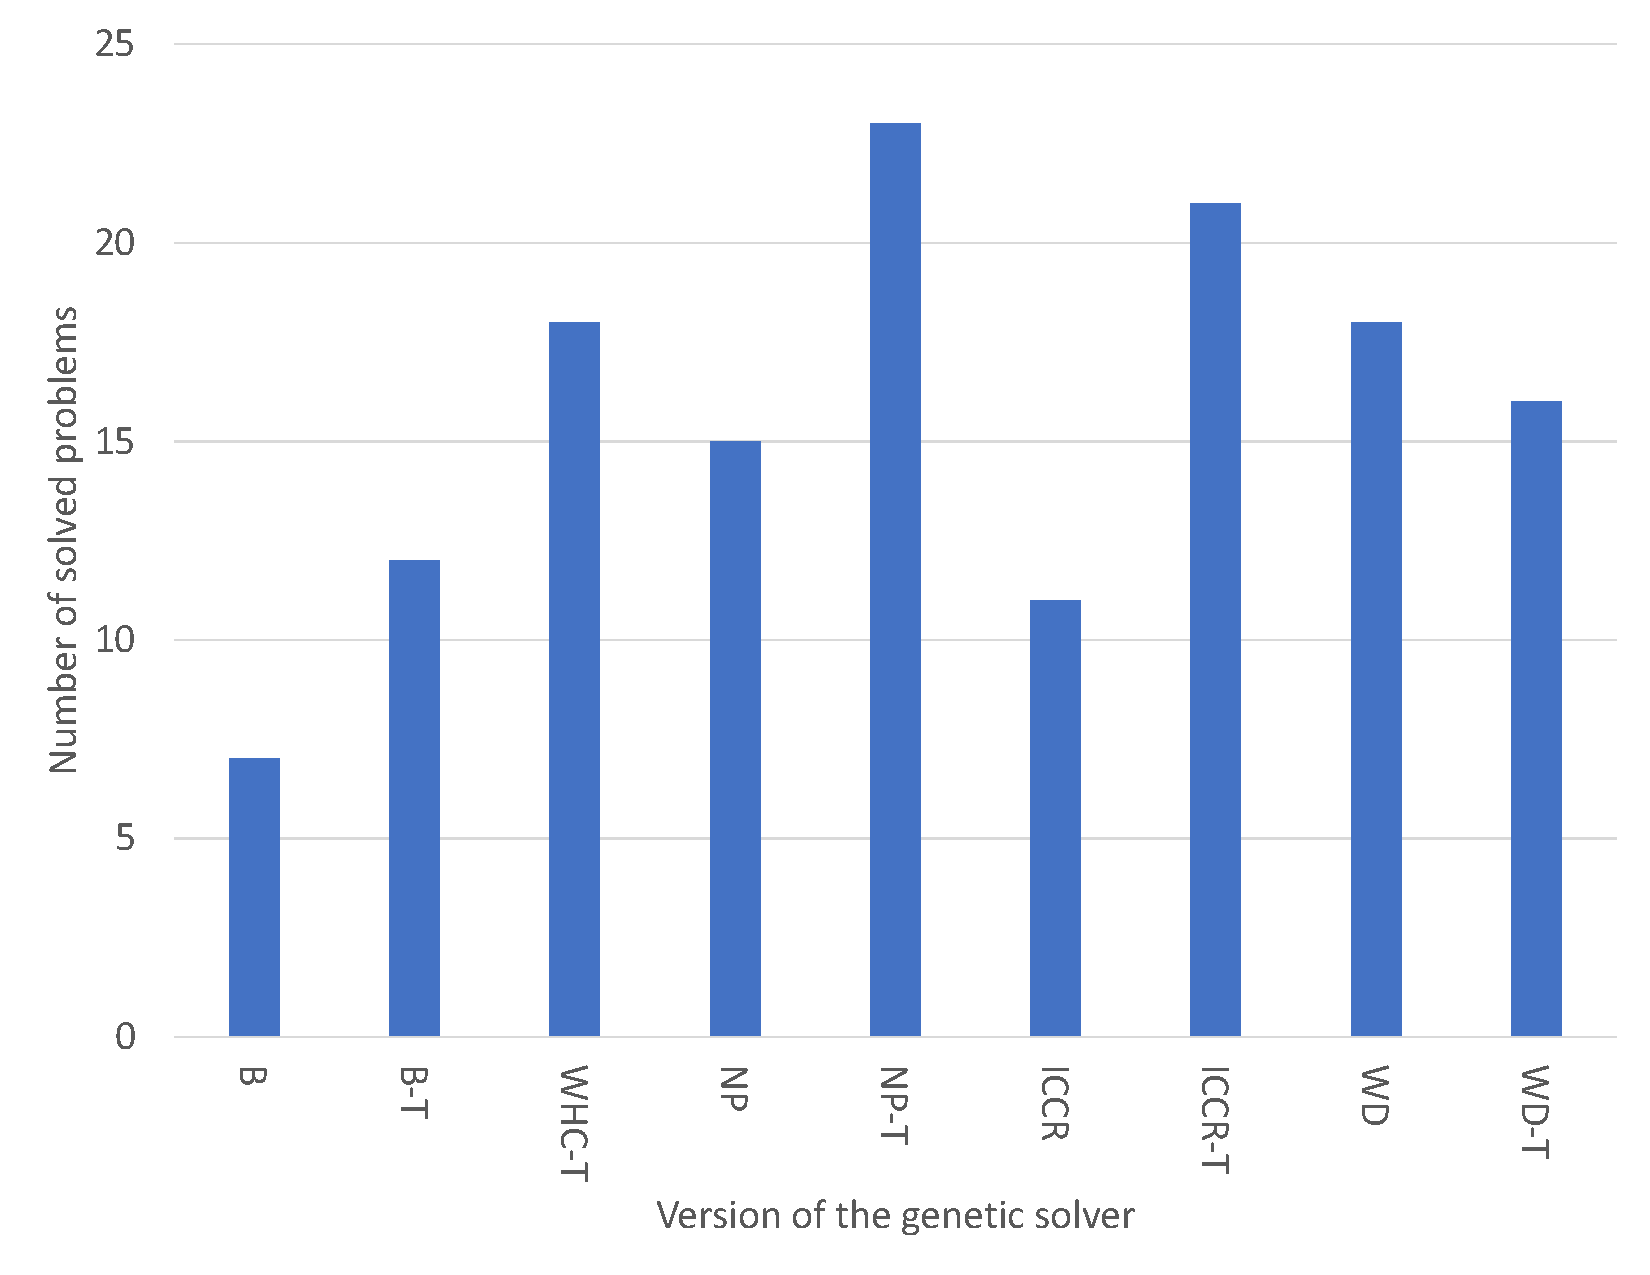
\includegraphics[width=\textwidth]{images/EvaluationNumberOfSolvedProblems.pdf}
	\caption[Number of problems for each version of the genetic solver]{Number of solved problems for each version of the genetic solver}
	\label{fig:EvaluationNumberOfSolvedProblems}
\end{figure}

Figure~\ref{fig:EvaluationNumberOfSolvedProblems} shows the results of the benchmark. For each version of the genetic solver, a vertical bar is build. The height of the bar shows the number of solved problems from the benchmark set. 

The \textbf{B} version solved the least number of problems than any other version. Almost in all cases, parameter tuning increases the number of solved problems. It also confirms the answer to \textbf{RQ1}. 

The comparison of \textbf{B-T}, \textbf{WHC-T}, and \textbf{NP} versions shows that the \textbf{NP} bar is higher than \textbf{B-T} but lower than \textbf{WHC-T}. This comparison confirms the first conclusion from Section~\ref{sec:NP}, that well-designed parameters are important for any algorithm. The combination of parameter engineering and parameter tuning in \textbf{NP-T} gives the best results. The same situation was observed for one problem in the previous chapter~(Figure~\ref{fig:boxplotsolverNoDuplicates}). 

Figure~\ref{fig:EvaluationNumberOfSolvedProblems} shows the results of the benchmark. For each version of the genetic solver, a vertical bar is build.

The benchmark also shows that no version of the genetic solver solves all problems from the set~(See Appendix~\ref{appendix:ProblemSet}). Table~\ref{tab:ProblemsColorCoding} shows the results of the benchmark in the context of a solved or unsolved problem. Each row describes the result of a specific problem. The column \textit{Problem Id} contains problem numbers. Black filled cell means that solver solved the problem. Table~\ref{tab:ProblemsColorCoding} also shows ids of problems that were not solved by all versions of the genetic solver.

Unsolved problems are presented in Table~\ref{tab:UnsolvedProblems}. It shows parameters that specified the problem. We can see there exist a few types of unsolved problems. All versions of the genetic solver could not solve the problem that contains 2 or more requests, and the depth of the tree is 3 or more. The exception is problem number 30. It has 1 request and depth equal to 4, but it also has 4 variants, and 100 resources and genetic solvers could not solve it. 

The depth of the tree has the most significant impact since it exponentially increases the number of nodes. As a result, there are more possible mappings between the software components and hardware resources. Other parameters with higher value give little increase in the number of possible combinations.

\begin{table}
	\centering
	\caption{Not solved problems}\label{tab:UnsolvedProblems}
	\resizebox{\textwidth}{!}{
		\begin{tabular}{c c c c c}
			\hline
			Problem Id & Software variants & umber of requests & Component tree depth & Resources ratio \\
			\hline            
			6 & 2 & 2 & 4 & 50 \\
			8 & 2 & 4 & 3 & 50 \\
			9 & 2 & 4 & 4 & 50 \\
			15 & 2 & 2 & 4 & 100 \\
			17 & 2 & 4 & 3 & 100 \\
			18 & 2 & 4 & 4 & 100 \\
			24 & 4 & 2 & 4 & 50 \\
			26 & 4 & 4 & 3 & 50 \\
			27 & 4 & 4 & 4 & 50 \\
			30 & 4 & 1 & 4 & 100 \\
			33 & 4 & 2 & 4 & 100 \\
			35 & 4 & 4 & 3 & 100 \\
			36 & 4 & 4 & 4 & 100 \\
			\hline
		\end{tabular}
	}
\end{table}

If a genetic solver could solve some problems, then solutions have a quality.
Let us now discuss the quality of the received results. Figure~\ref{fig:EnergyPercentage} shows the percentage of the deviation from the optimum for problems that solved by all versions of the genetic solver. The optimum values for problems were received by the \textbf{ILP} solver. If the percentage of the deviation is zero, that means that the received solution is \textbf{optimal}. The max deviation is near 30\% for the B version with problem 31. However, other versions give solutions with deviation from optimal that less than 10\% or even optimal solutions for the \textbf{NP-T} version. There are high deviations from optimum in problems number 13 for tuned versions of the genetic solver such as \textbf{B-T}, \textbf{NP-T}, \textbf{ICCR-T}, and \textbf{WD-T}. Nevertheless, \textbf{WHC-T} and untuned versions give a near-optimal solution with minimal deviation. The \textbf{ICCR} version gives a much higher percentage of deviation than other versions in problem 19.

\begin{figure}
	\centering
	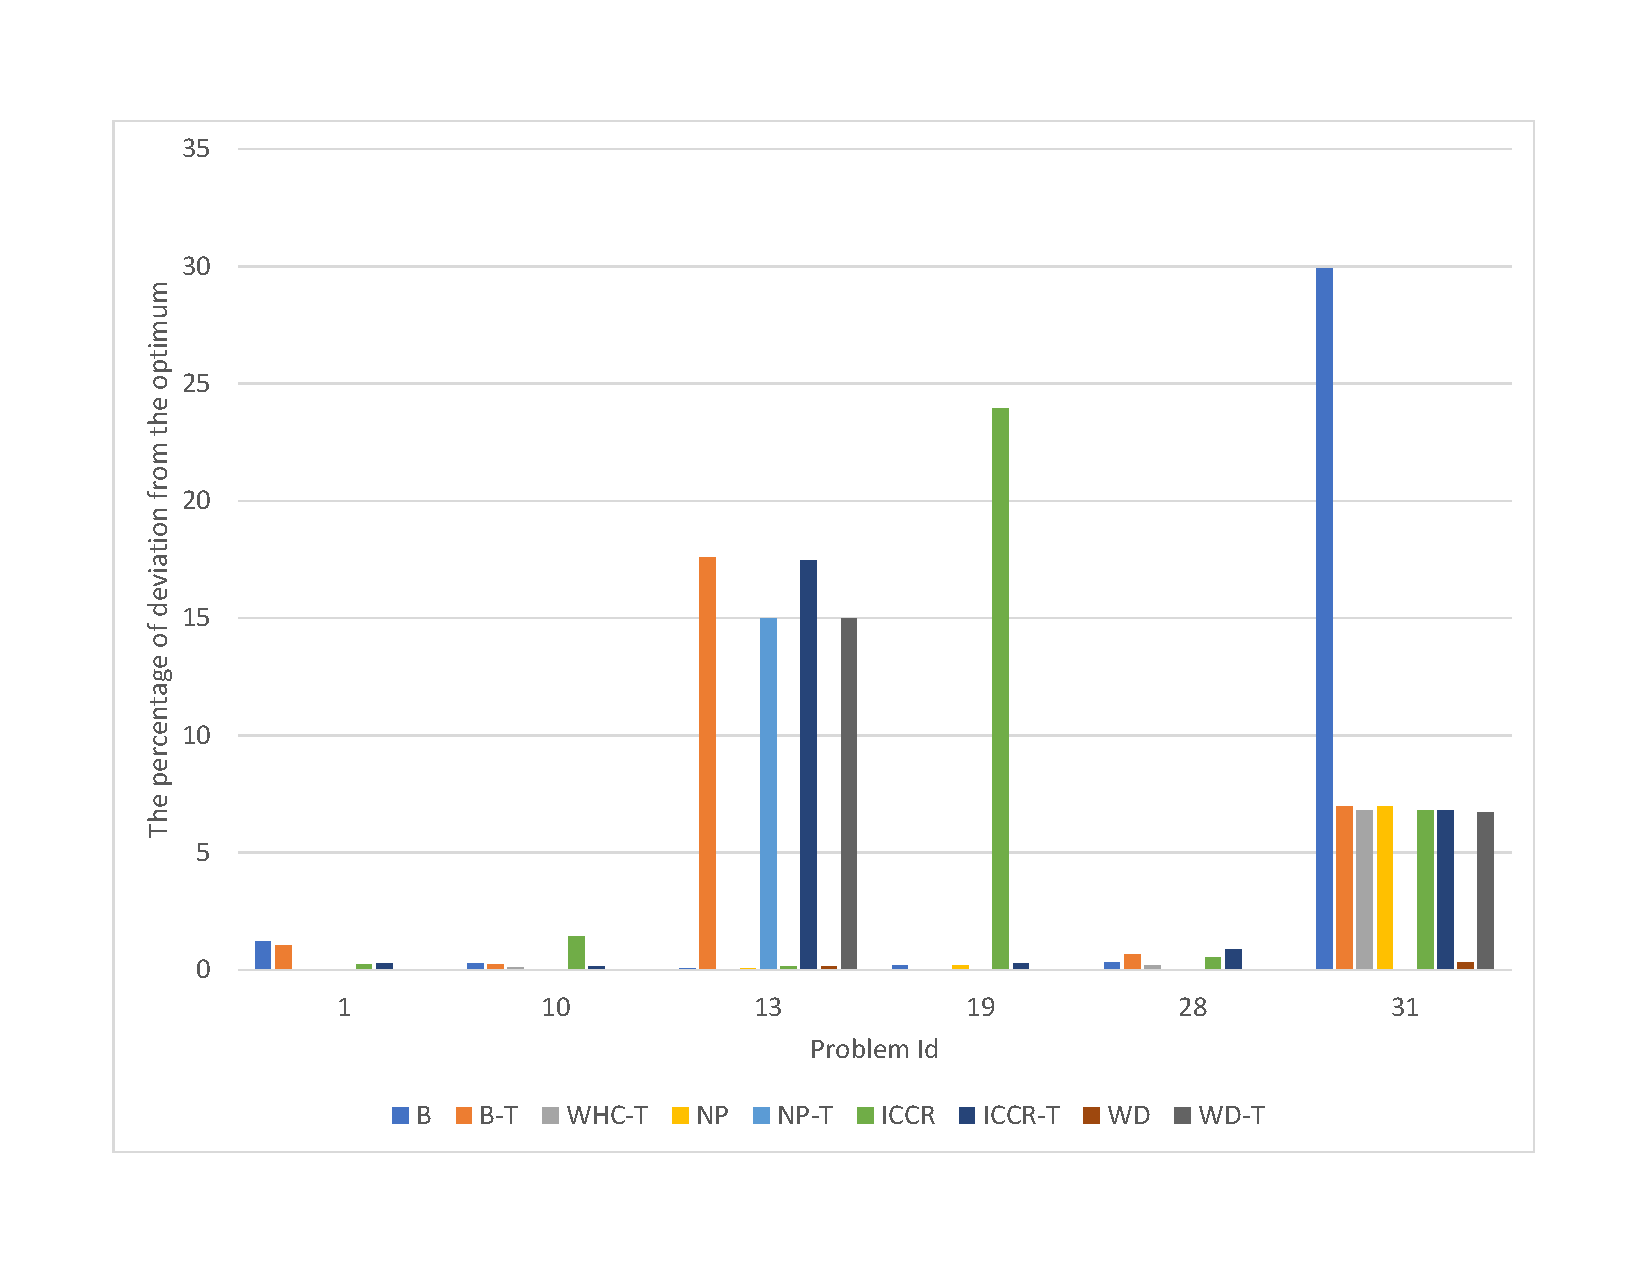
\includegraphics[width=\textwidth]{images/EnergyPercentage.pdf}
	\caption[The deviation from the optimum of solved by all solvers problems]{The deviation from the optimum of solved by all solvers problems}
	\label{fig:EnergyPercentage}
\end{figure}

Figure~\ref{fig:EnergyPercentage} also shows that the deviation is increasing for big size problems. To confirm that fact, we take two problems with different sizes~(Figures~\ref{fig:SmallMediumProblemEnergy}). These problems are solved by all versions of the genetic solver except the B version. Figure~\ref{fig:SmallProblemEnergy} shows the percentage of deviation from optimum for a small size problem. This problem's parameters are:
\begin{itemize}
	\item Software variants: 2;
	\item Number of requests: 2;
	\item Component tree depth: 2;
	\item Resources ratio: 50;
	\item Timeout to solve the problem: 5 minutes.
\end{itemize}

The quality of results for the problem is near-optimal because the deviation is less than one percent. The \textbf{NP-T} and \textbf{WD-T} versions give an optimal solution for the problem.

Figure~\ref{fig:MediumProblemEnergy} shows the percentage of deviation from optimum for a bigger size problem. This problem's parameters are:
\begin{itemize}
	\item Software variants: 4;
	\item Number of requests: 1;
	\item Component tree depth: 3;
	\item Resources ratio: 100;
	\item Timeout to solve the problem: 5 minutes.
\end{itemize}


The quality of results in a case of the bigger problem is much worse. The minimal deviation is 35\% for the \textbf{NP-T} version. The \textbf{WD} and \textbf{WD-T} versions give less number of valid solutions, but with better quality. The reason why the quality of solutions is decreasing with a bigger size of the problem could be a higher number of hardware resources. The higher number of resources means that more hardware resources could satisfy the requirements of the software component. The genetic solver could not find best-suited resources for requested components, and as a result, quality is decreasing. 


\begin{figure}
	\centering
	\begin{subfigure}{0.45\textwidth}
		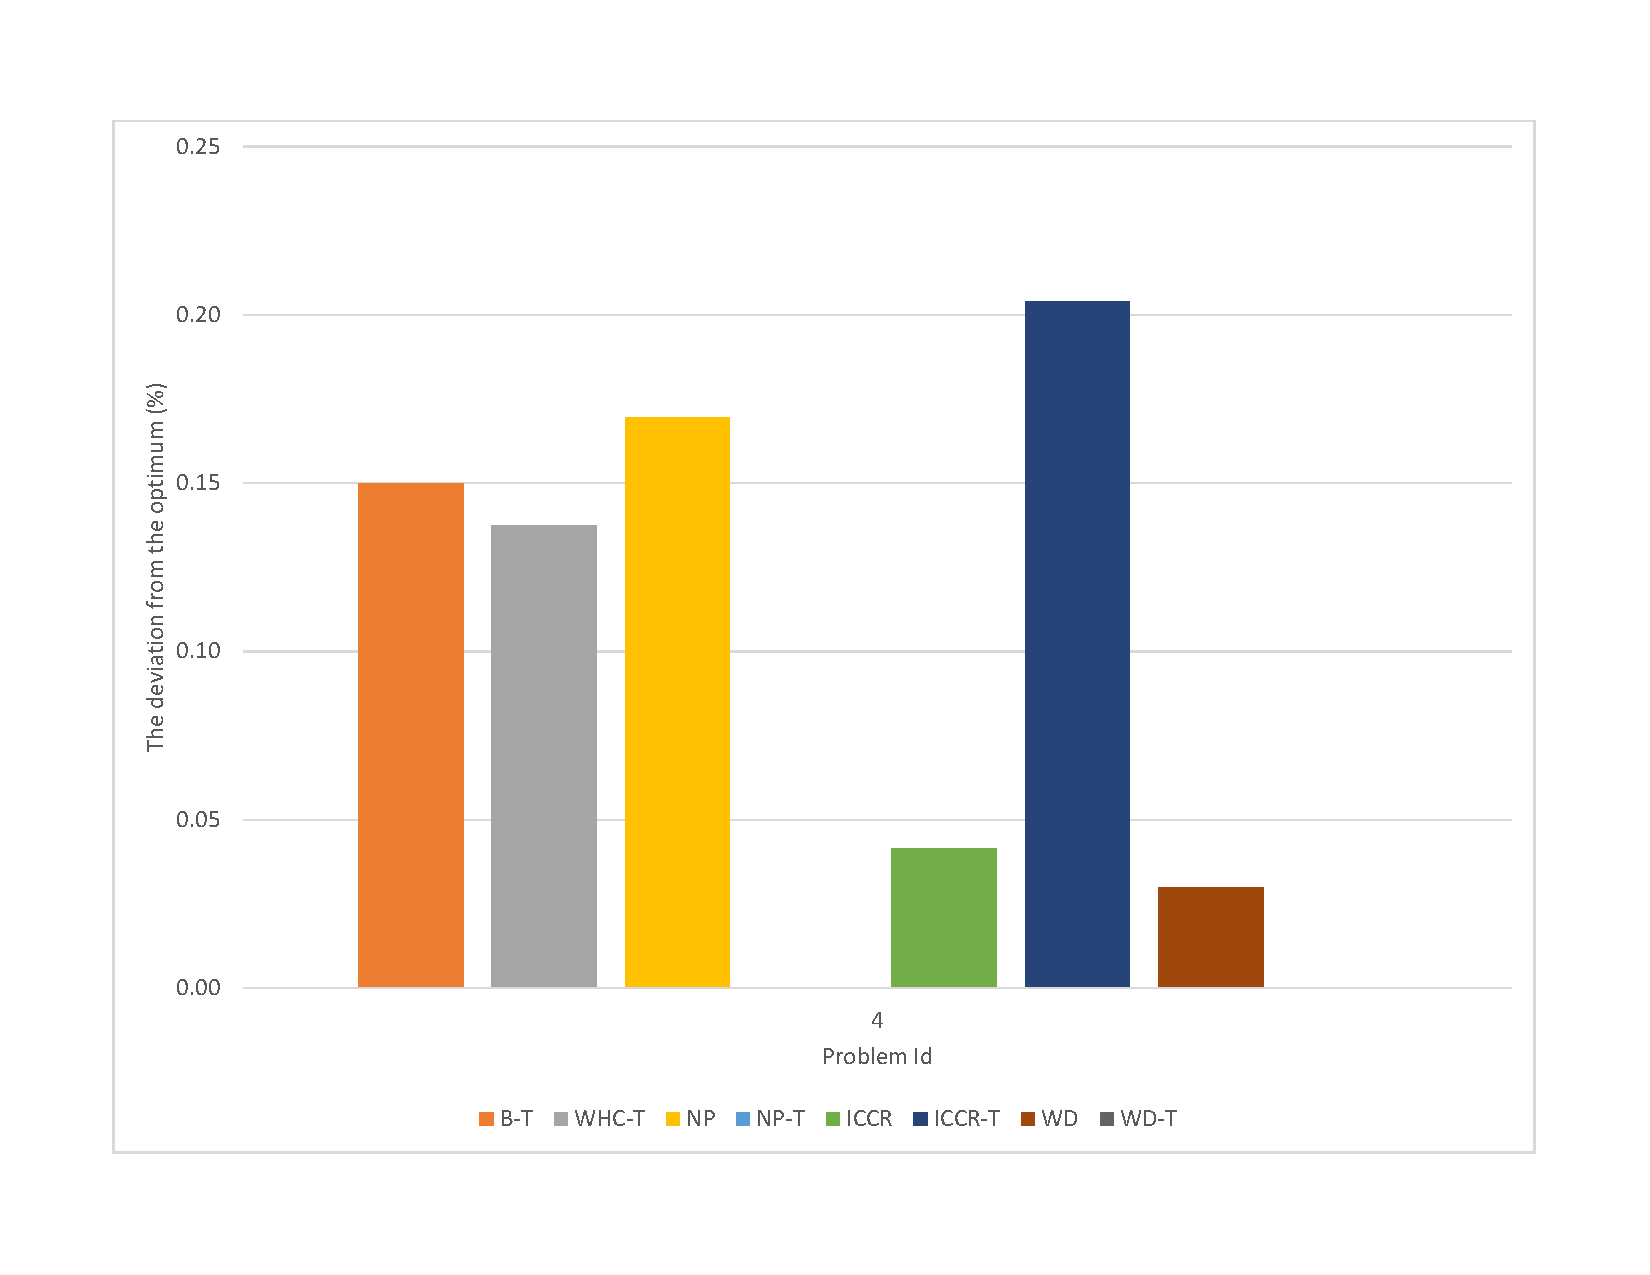
\includegraphics[width=\textwidth]{images/EnergyDeviationSmallProblem.pdf}
		\caption{Small sized problem}
		\label{fig:SmallProblemEnergy}
	\end{subfigure}
	\hfill
	\begin{subfigure}{0.45\textwidth}
		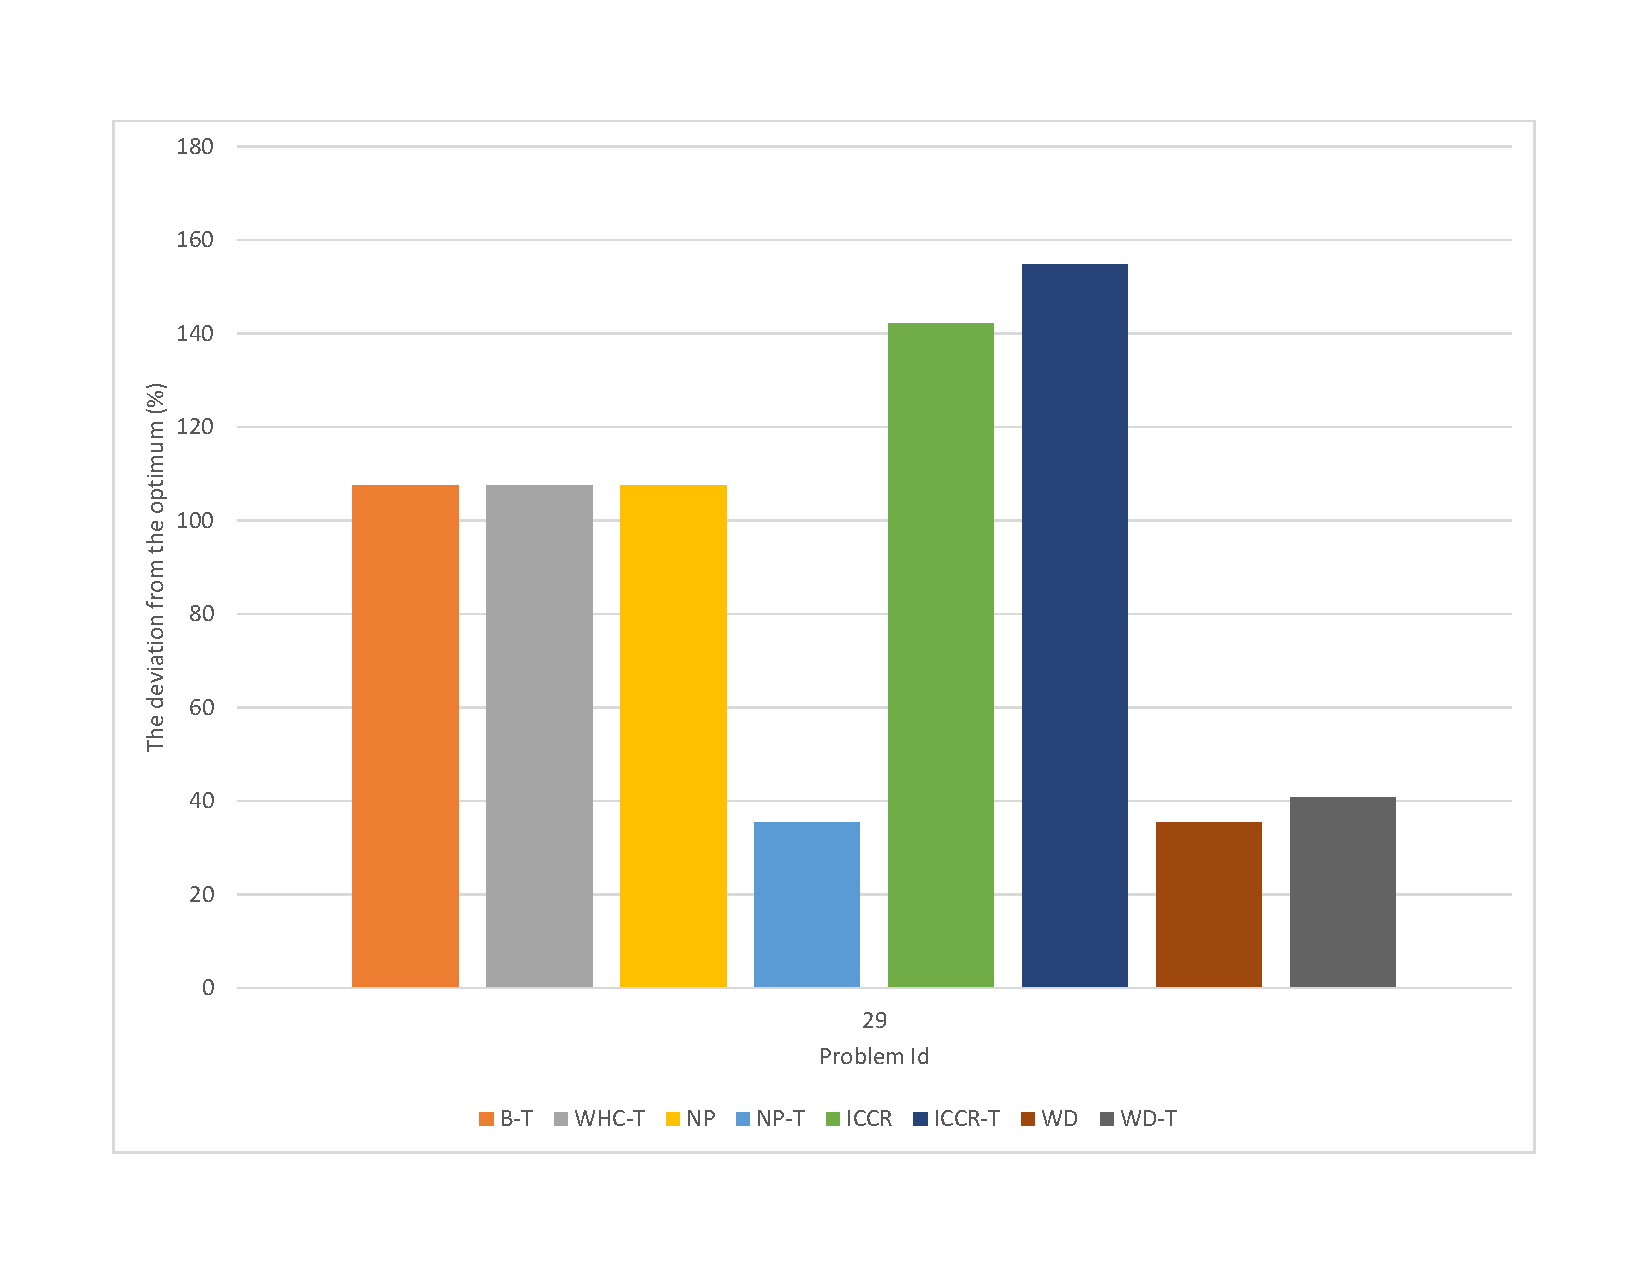
\includegraphics[width=\textwidth]{images/EnergyDeviationMediumProblem.pdf}
		\caption{Big sized problem}
		\label{fig:MediumProblemEnergy}
	\end{subfigure}    
	\caption[The deviation from the optimum for small and big sized problem]{The deviation from the optimum for small and big sized problem}
	\label{fig:SmallMediumProblemEnergy}    
\end{figure}


This section shows that our modifications improve the results of the genetic solver. The \textbf{NP-T} version solved \textbf{3 times more} problems than the \textbf{B} version. We evaluated the quality of solutions. As a result of the quality evaluation, we make two conclusions. First, the modified versions of the genetic solver also improve the quality of the results. Second, the quality is decreasing for bigger size problems.
However, there are problems from the set that the genetic solver can not solve.


\section{Analysis}

Benchmark showed that a genetic solver could not solve all MQuAT problems from the evaluation set.
In this section, we present a discussion of results and reasons why described in Chapter~\ref{chapter:Implementation} enhancements, and optimizations are not giving the desired efficiency.

Firstly, let us discuss the reasons why modifications improve the genetic solver. After that, we will describe the reasons why not all problems could be solved.

\paragraph{Positive reasons} \\
There are a few reasons why the genetic solver with our modifications could solve more problems than the \textbf{B} version. 

First, parameter tuning is performed for all versions of the genetic solver. Optimized values of parameters give better results, as it showed in the previous section. 

The second reason is in new probabilities that we added in Section~\ref{sec:NP}. These probabilities give a possibility to change the position of the crossover and mutation points randomly, but as a result, the genetic solver gives results that a bit worse than parameter tuning. 

\paragraph{Negative reasons} \\
There are a few reasons why not all problems are solved.

One of the reasons for such a result is that we optimized parameters for a specific problem that we described at the beginning of Chapter~\ref{chapter:Implementation}.

Obtained results could be explained with a \textbf{"no free lunch" (NFL) theorem}~\cite{wolpert1996, wolpert1997}. It states that if an algorithm is performing well with a certain class of tasks, then it must pay for it with a deterioration in performance on the set of all remaining problems.

Another reason that we optimize parameters without knowledge about dependencies between them. Parameters that we found or added did not fit well for our goals. Let us analyze earlier discussed parameters.

\subsection{Search Space}

We start the analysis by determining the search space structure. We perform measurements for more than three thousand configurations using BRISE in the Search space exploration mode with the NP version of the genetic solver. This mode was described in Section~\ref{sec:BRISE}. For this type of analysis, we use the same problem as in Chapter~\ref{chapter:Implementation} and it has following properties:
\begin{itemize}
	\item Software variants: 10;
	\item Number of requests: 15;
	\item Component tree depth: 2;
	\item Resources ratio: 5.
\end{itemize}

The search space for the SPEA2 selector as a parallel coordinates plot is shown in Figure~\ref{fig:SearchSpaceViewFull}.
Each vertical line represents a parameter, its values range. Each measured configuration is shown on the plot as a line that connects parameter values for the Genetic Solver. The last vertical line, as well as the color, indicates the number of contract violations that the configuration gives. The more dark color means fewer contract violations and vise versa, the configuration with lighter color gives a higher number of contract violations.

\begin{figure}
	\centering
	\includegraphics[width=\textwidth]{images/SPEA2.pdf}
	\caption[Search space representation]{Search space representation}
	\label{fig:SearchSpaceViewFull}
\end{figure}

Figure~\ref{fig:SearchSpaceViewFull} shows that all values of parameters could give "good" and "bad" results. There are no visible dependencies between parameters. 

\begin{figure}
	\centering
	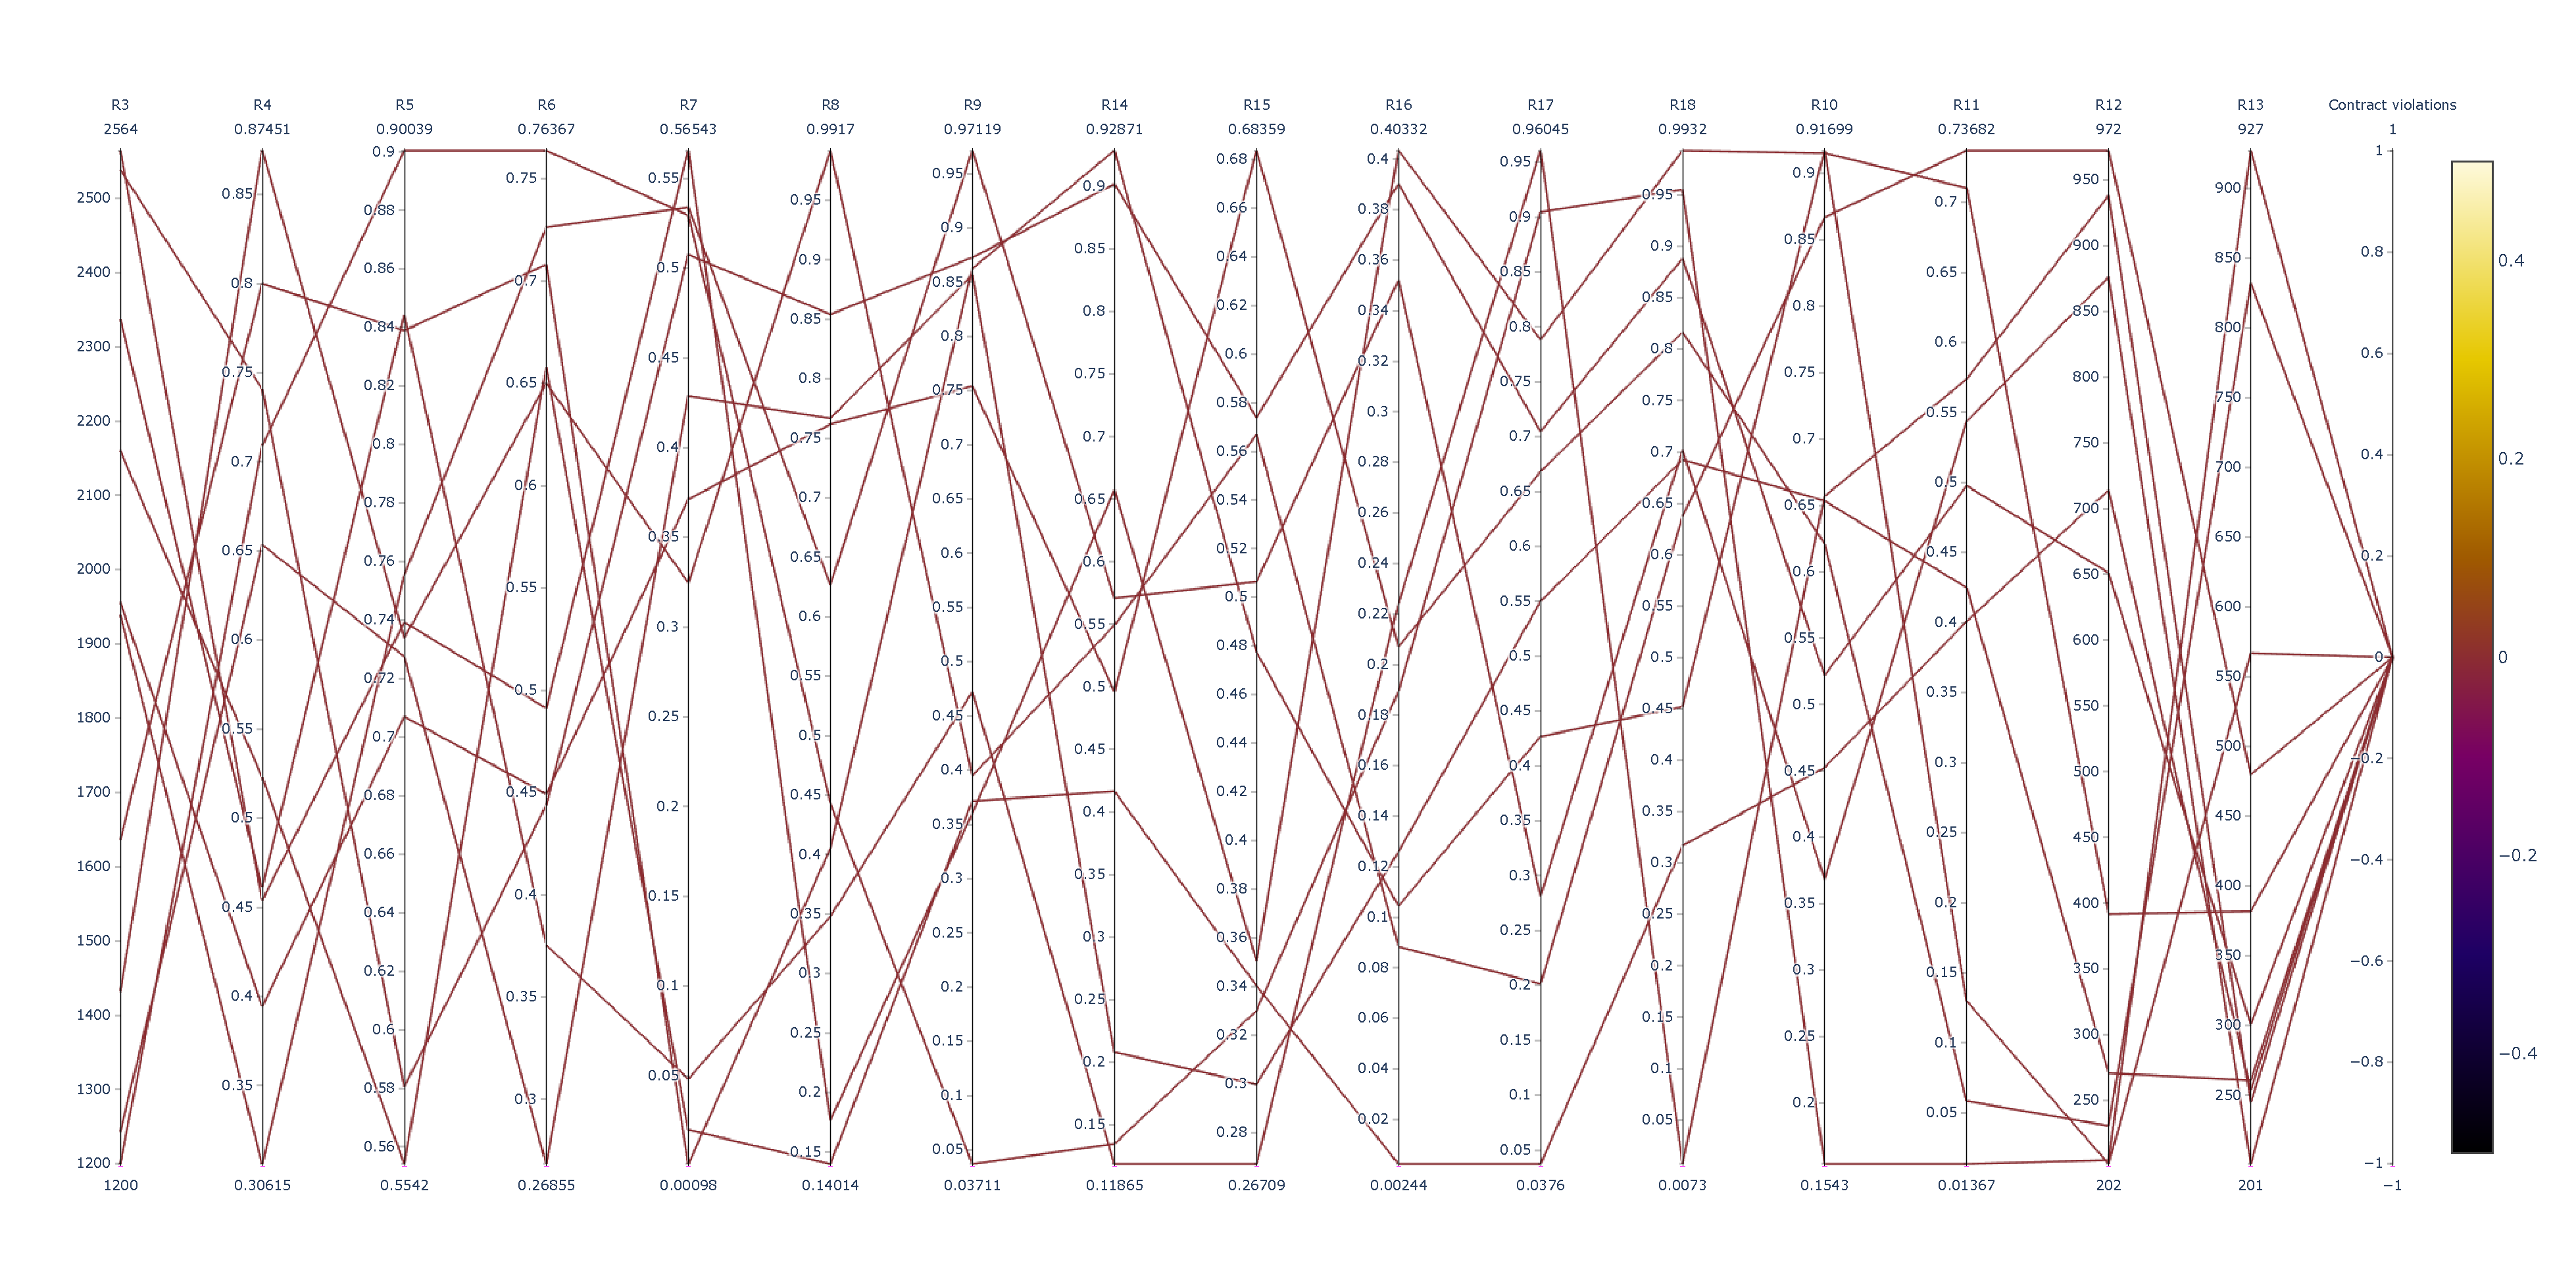
\includegraphics[width=\textwidth]{images/SPEA2_Zero_validity.html.pdf}
	\caption[Search space representation of valid results]{Search space representation of valid results}
	\label{fig:SearchSpaceValid}
\end{figure}

If we filter out all configurations that give not valid results, we get the search space with a few configurations. Figure~\ref{fig:SearchSpaceValid} demonstrates these configurations. As shown, there are ranges of values that give valid results. Parameters such as R4 and R5 have the range on the higher values. However, R16 needs to be smaller.

\begin{figure}
	\centering
	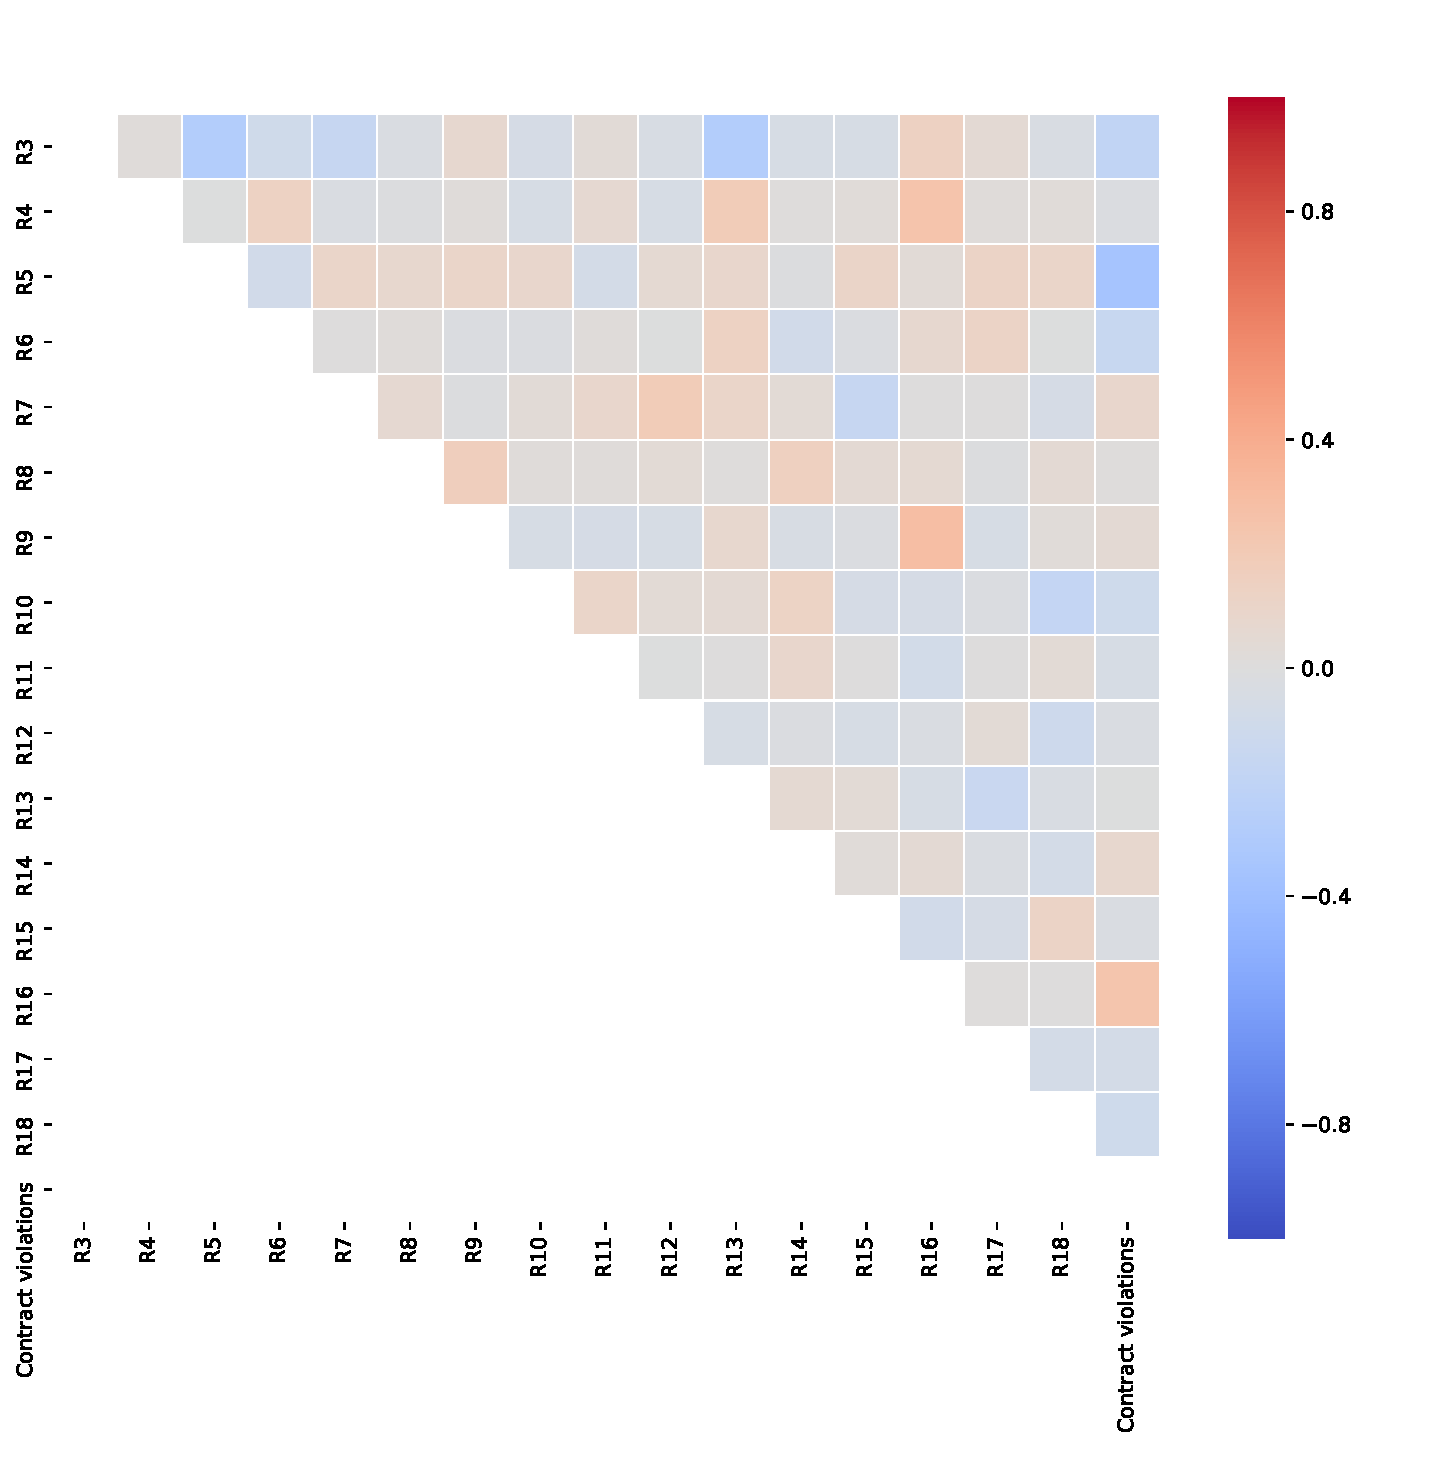
\includegraphics[width=\textwidth]{images/CorrelationAnalysis.pdf}
	\caption[Correlation analysis matrix]{Correlation analysis matrix}
	\label{fig:CorrelationAnalysis}
\end{figure}

Since Figure~\ref{fig:SearchSpaceViewFull} and Figure~\ref{fig:SearchSpaceValid} show that the search space is very complex, we perform another method of analysis to analyze dependencies between parameters.

\subsection{Correlation Analysis}

We perform the correlation analysis of parameters to understand how they rely on each other. Figure~\ref{fig:CorrelationAnalysis} shows the results as a correlation matrix where the intensity of the correlation is the color of the cell. The more intense color means a stronger correlation. Each row and column in this matrix represent the parameter of the genetic algorithm. We display only an upper triangle of the matrix because it is symmetric. The last column of the matrix represents the correlation between parameters of the genetic solver (NP version) and a number of contract violations~(CVs). There are two types of correlation. A direct correlation has a red color, and an inverse correlation has a blue color. In the case of correlation to CVs, direct correlation means that a bigger value o parameter gives a bigger number of contract violations. Inverse correlation, in the same case, means that the bigger value of parameter gives a smaller number of contract violations. Grey color shows that there is no correlation.

From the correlation analysis, we can conclude that there are no strong dependencies between the number of contract violations and parameters. There are two more important parameters: \texttt{CrossoverRate}~(R5) and \texttt{Cross\-ov\-er\-On\-Ran\-dom\-Re\-qu\-est\-Pro\-ba\-bi\-li\-ty}~(R16).
The analysis showed that the \texttt{CrossoverRate} parameter needs to have big value and value of \texttt{Cross\-ov\-er\-On\-Ran\-dom\-Re\-qu\-est\-Pro\-ba\-bi\-li\-ty} needs to be as low as possible. In this case of the small value of probability, it may be a good idea to remove this parameter for parameter tuning.

Correlation analysis shows that some parameters have dependencies. Nevertheless, we do not know yet how they depend.

\subsection{Parameter Pairs Distributions}

For further investigation of dependencies, we construct plots that demonstrate all parameter values of two different parameters.
Each point on the plot is a combination of two parameter values. We are calling them as distribution of parameter pairs. We will discuss only two distribution. The first plot will show one particular distribution, and the second plot represents how most of the constructed distributions look like.

\begin{figure}
	\centering
	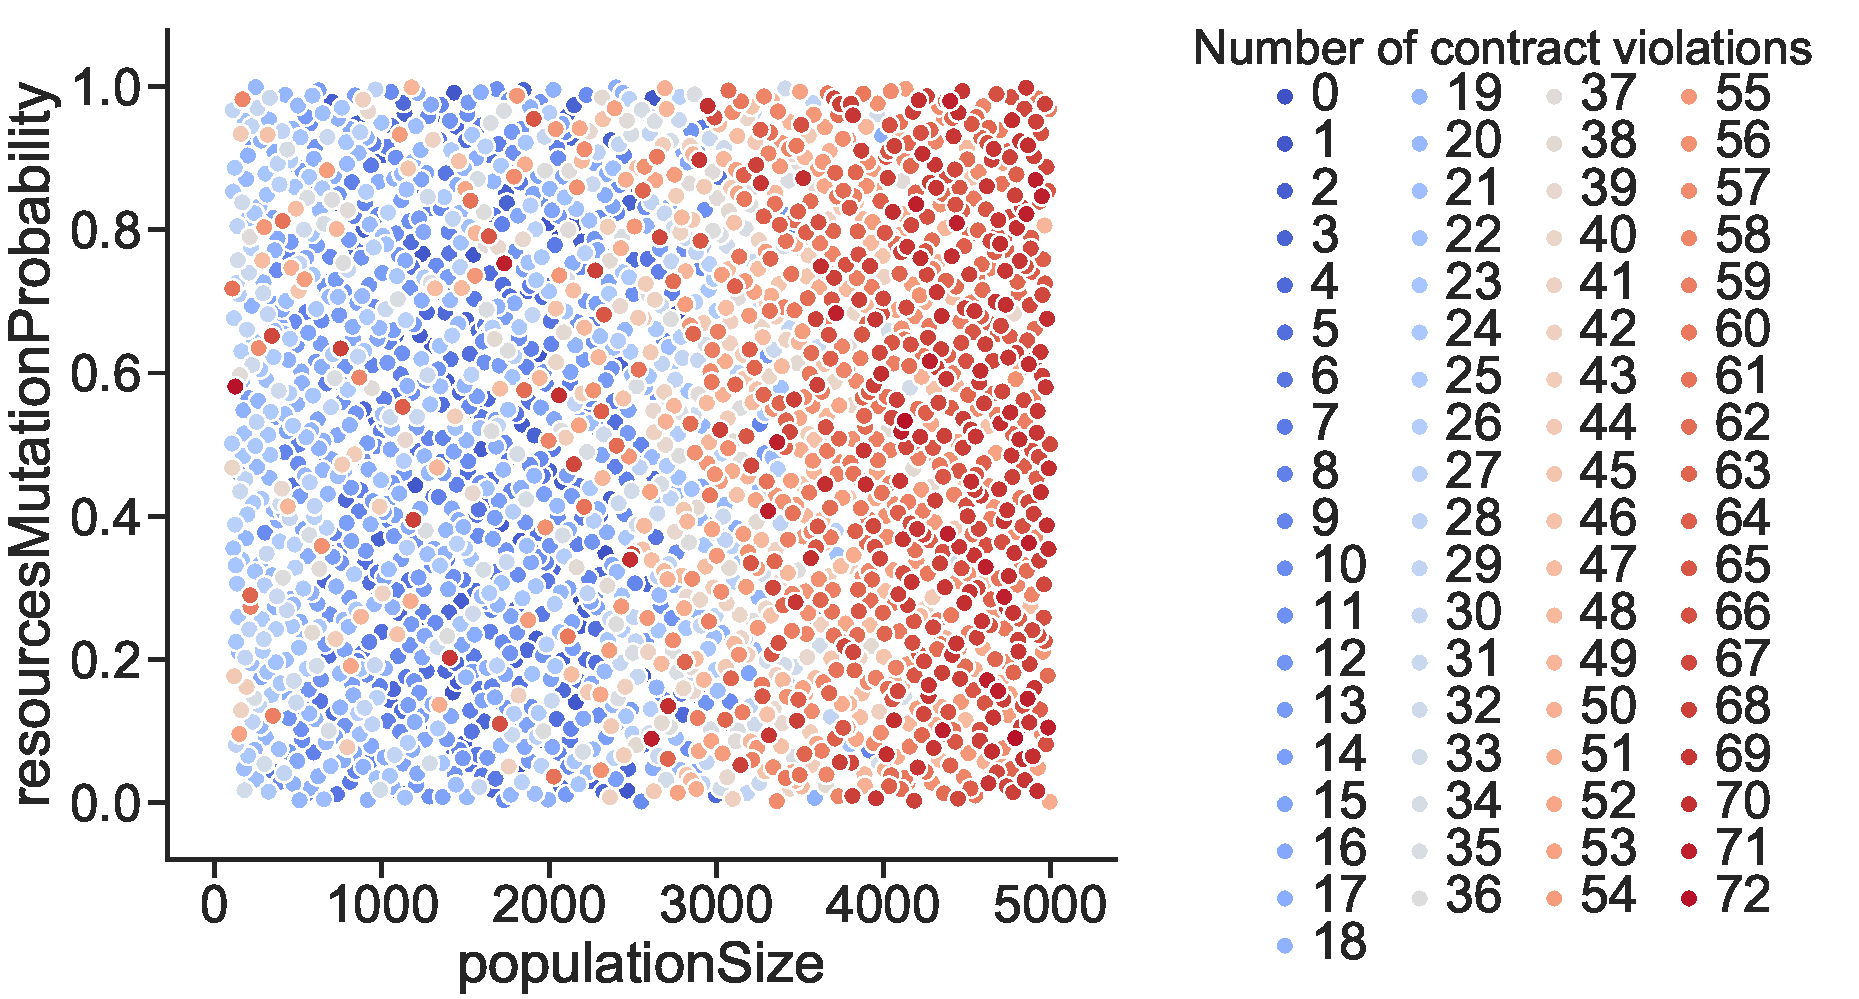
\includegraphics[width=\textwidth]{images/populatioSizeVsResMutationProbability.pdf}
	\caption[Parameter pair distribution of \texttt{populatioSize}~(R3) and \texttt{re\-so\-ur\-ces\-Mu\-ta\-ti\-on\-Pro\-ba\-bi\-li\-ty}~(R8)]{Parameter pair distribution of \texttt{populatioSize}~(R3) and \texttt{re\-so\-ur\-ces\-Mu\-ta\-ti\-on\-Pro\-ba\-bi\-li\-ty}~(R8)}
	\label{fig:populatioSizeVsResMutationProbability}
\end{figure}

Figure~\ref{fig:populatioSizeVsResMutationProbability} shows the representative distribution. Each point on this plot represent a value combination of two parameters \texttt{populationSize}~(R3) and \texttt{re\-so\-ur\-ces\-Mu\-ta\-ti\-on\-Pro\-ba\-bi\-li\-ty}~(R8). The color of the point is the number of contract violations. In this case, blue color is a small number of contract violations. Red color represents a big number of contract violations. As we can see, there is gradient coloring from the mostly blue on the left size to mostly red on the right size. Such result means that \texttt{po\-pu\-la\-ti\-on\-Si\-ze}~(R3) have a bigger influence on the result than \texttt{re\-so\-ur\-ces\-Mu\-ta\-ti\-on\-Pro\-ba\-bi\-li\-ty}~(R8). The figure also shows that for any value of \texttt{re\-so\-ur\-ces\-Mu\-ta\-ti\-on\-Pro\-ba\-bi\-li\-ty}~(R8), there are results with any number of contract violations.

\begin{figure}
	\centering
	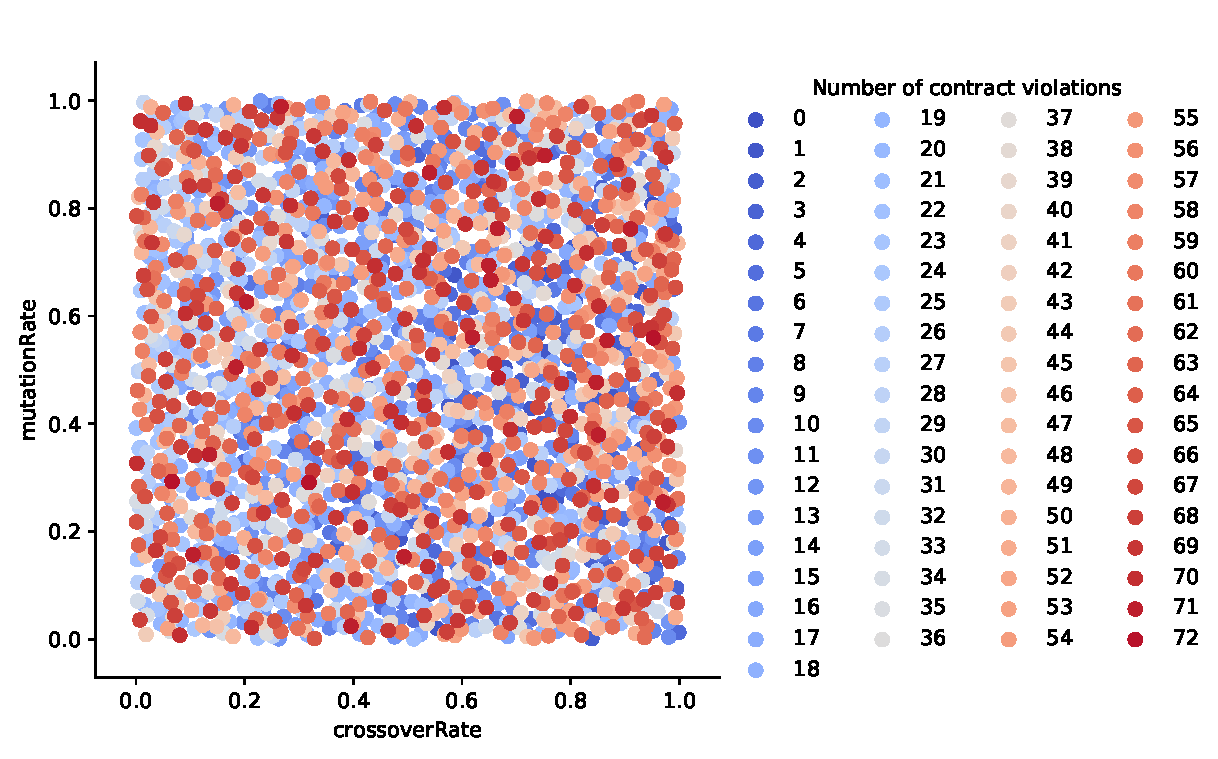
\includegraphics[width=\textwidth]{images/CrossoverRateVsutationRate.pdf}
	\caption[Parameter pair distribution of \texttt{CrossoverRate}~(R5) and \texttt{mutationRate}~(R7)]{Parameter pair distribution of \texttt{CrossoverRate}~(R5) and \texttt{mutationRate}~(R7)}
	\label{fig:CrossoverRateVsMutationRate}
\end{figure}

However, most distributions look like the distribution of \texttt{crossoverRate}~(R5) and \texttt{mutationRate}~(R7). It is showed in Figure~\ref{fig:CrossoverRateVsMutationRate}. As we can see, "good" and "bad" results scatter over all values of the described parameters. That means that these parameters do not depend on each other.

Distributions of combinations of two parameters shows that some parameters have a more significant impact on the result than others. Moreover, there are parameters on the value of which the result does not depend. More examples of such distributions showed in Appendix~\ref{appendix:Distributions1}.

\subsection{Parameter Values Distributions in Terms of Contract Violations}

\begin{figure}
	\subfloat[Bigger sized problem]{%
		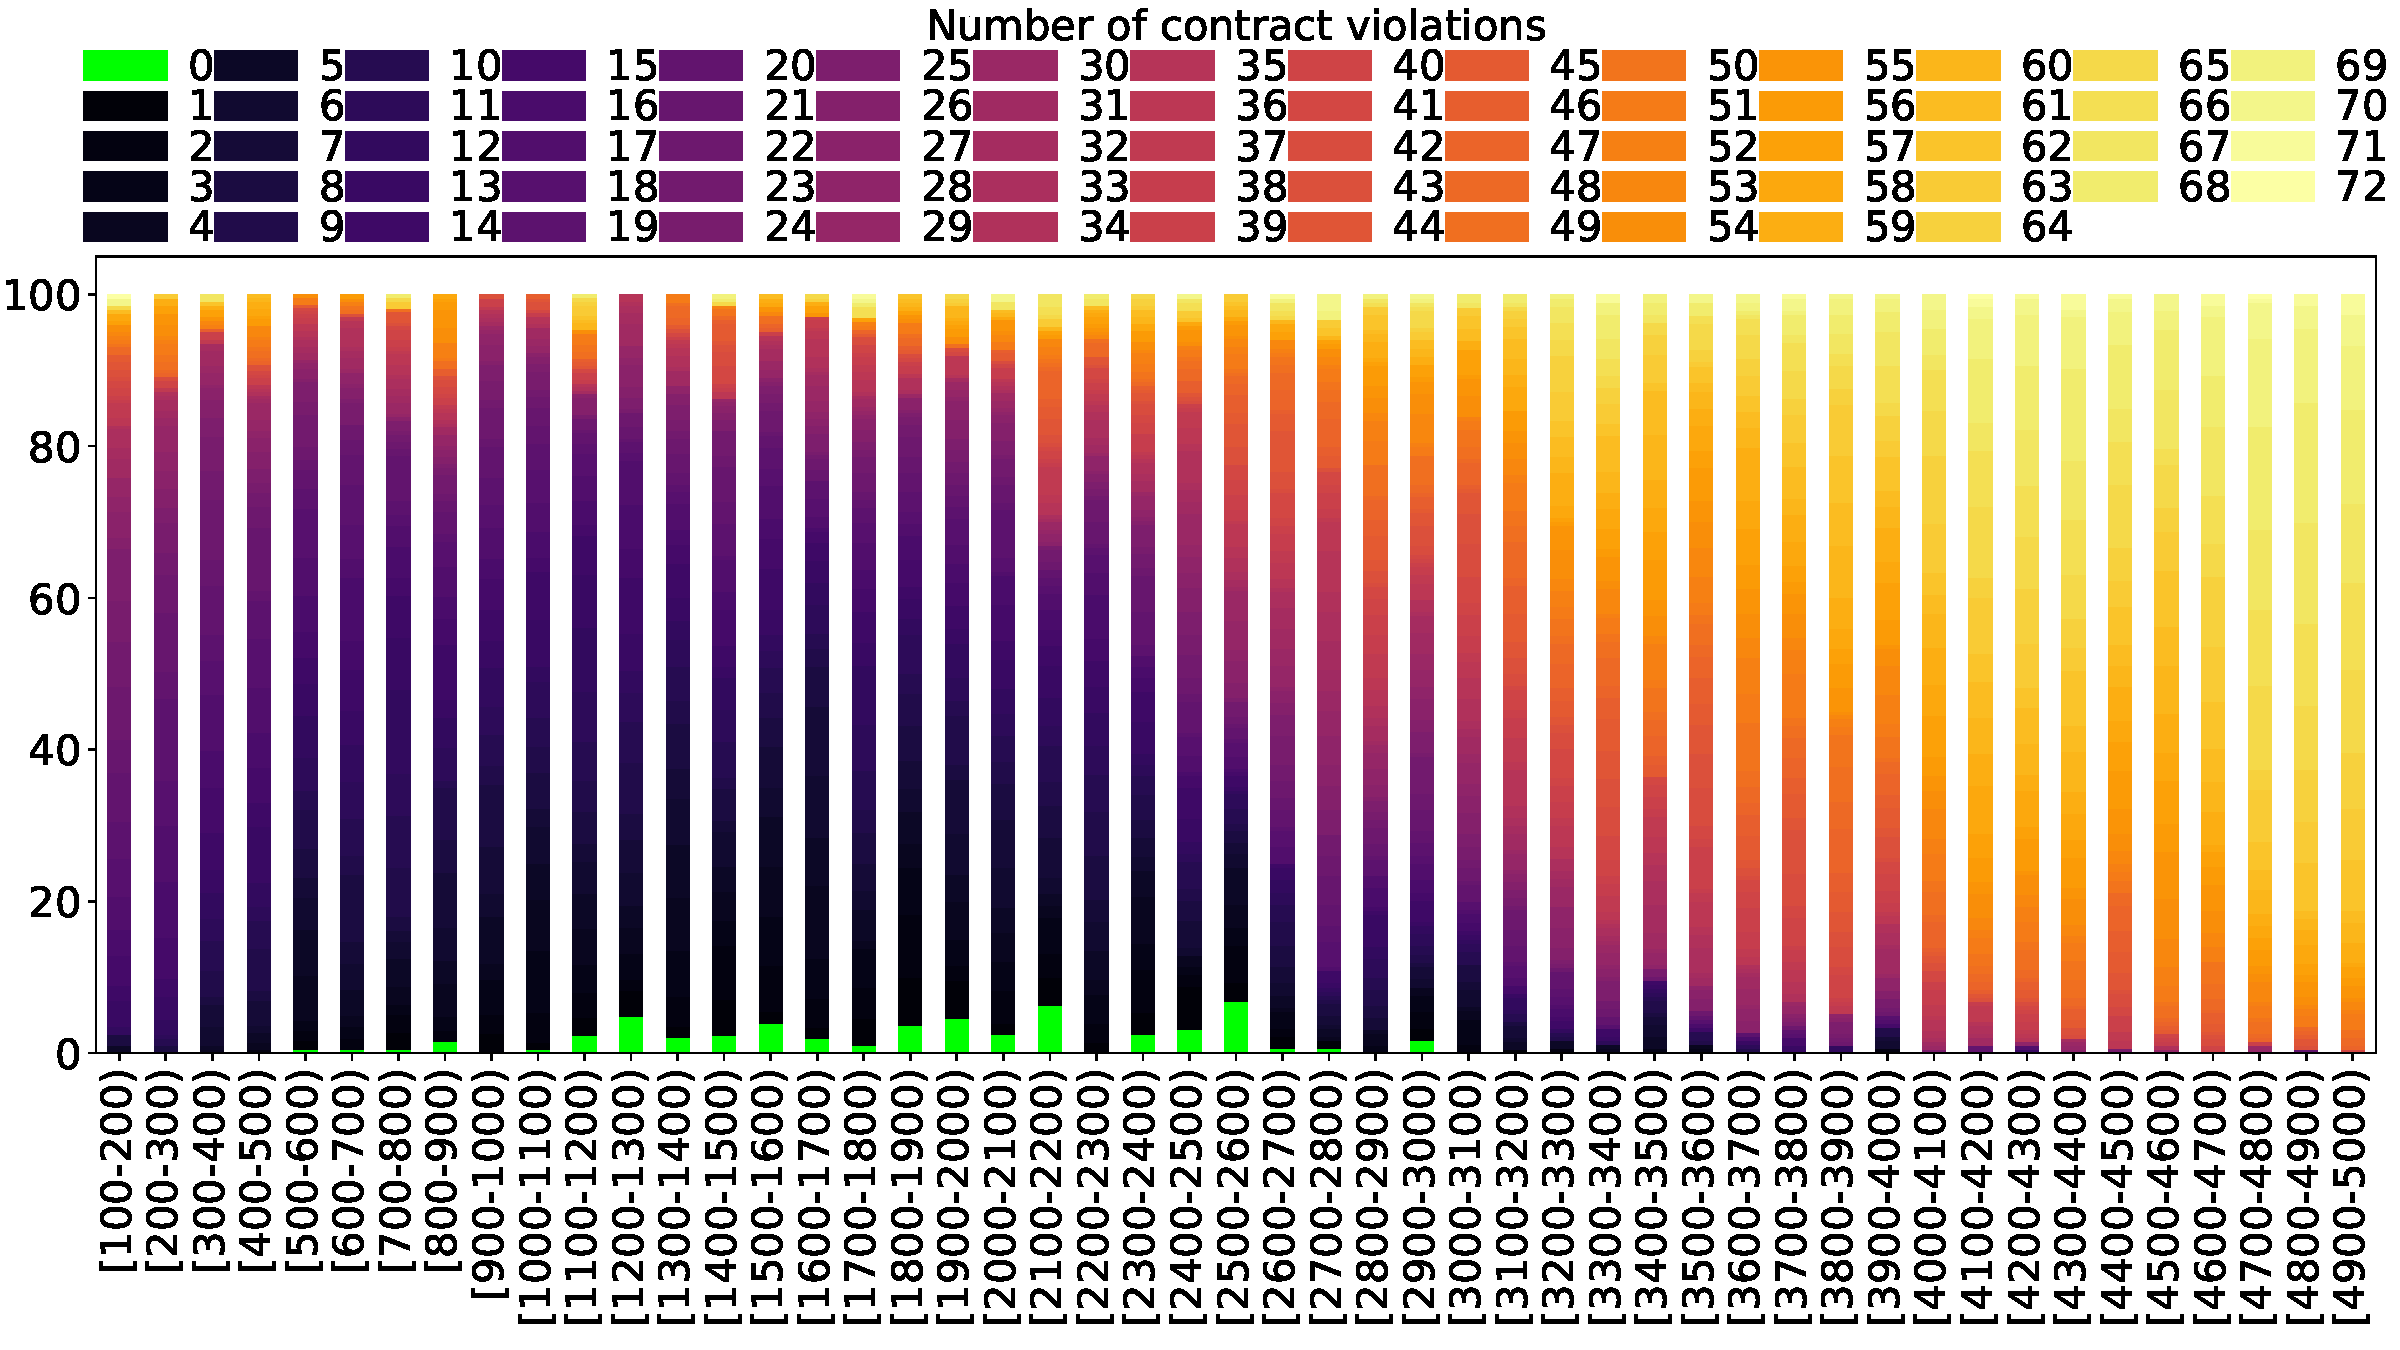
\includegraphics[clip,width=\textwidth]{images/populationSize_gradientBig.pdf}%
		\label{fig:populationSize_gradientBig}
	}
	\\
	\subfloat[Smaller sized problem]{%
		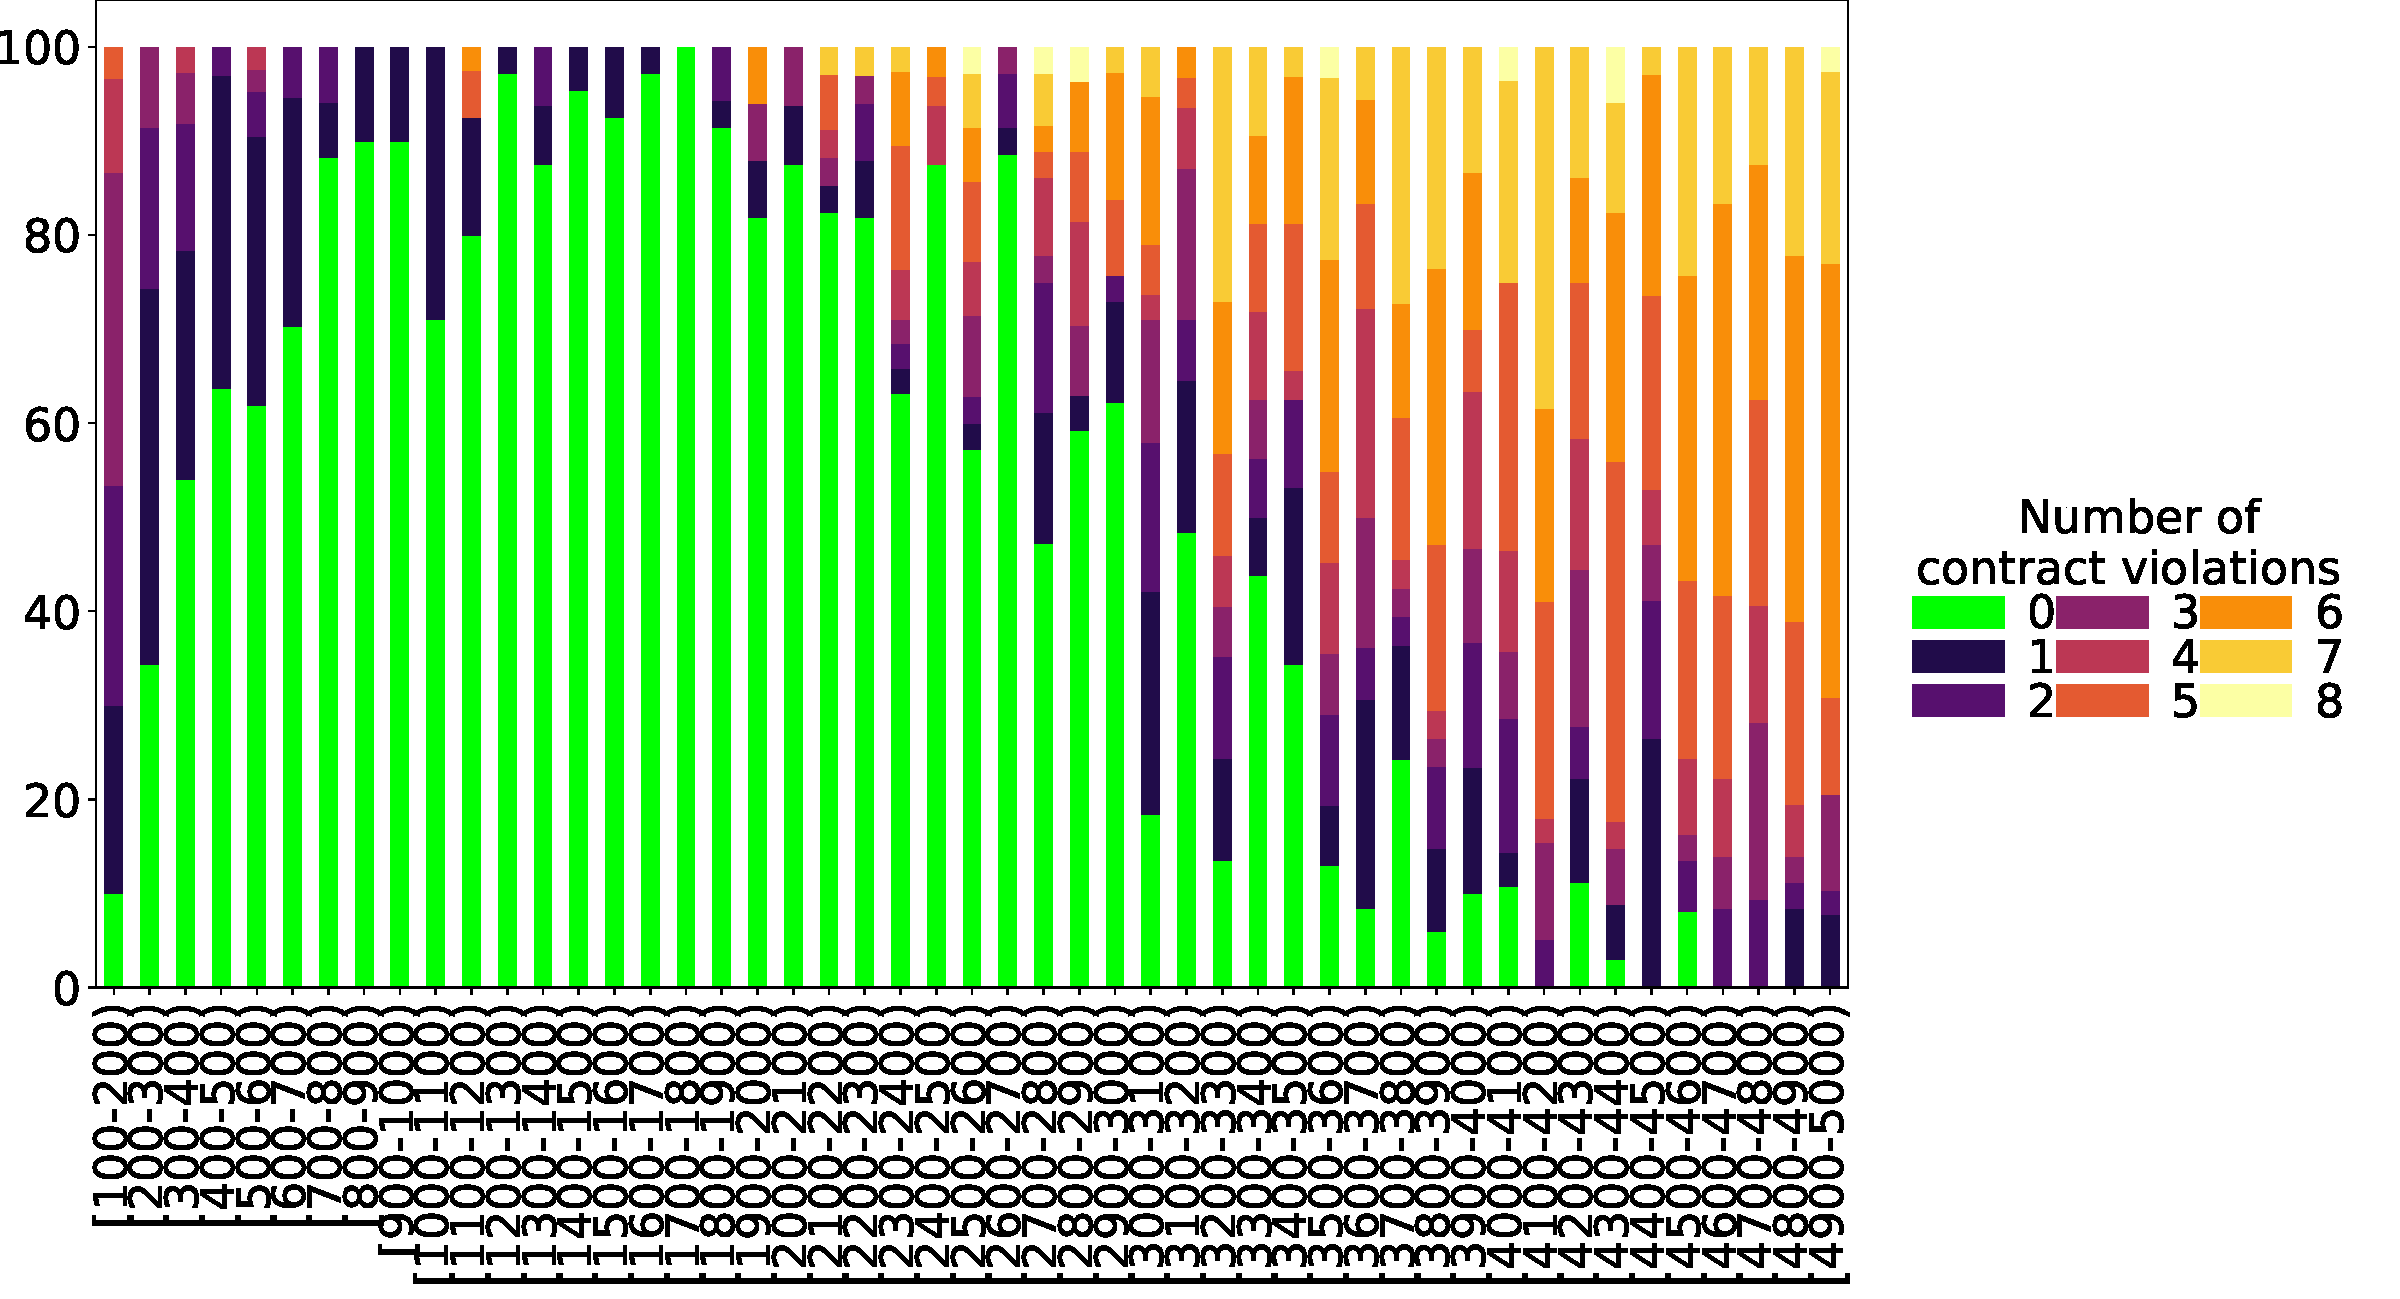
\includegraphics[clip,width=\textwidth]{images/populationSize_gradientSmall.pdf}%
		\label{fig:populationSize_gradientSmall}
	}
	
	\caption[\texttt{populationSize}~(R3) parameter values distribution of two problems in terms of contract violations]{\texttt{populationSize}~(R3) parameter values distribution of two problems in terms of contract violations}
	\label{fig:populationSize_gradient}
\end{figure}



Previously discussed plots show that the results quality of the genetic solver highly depends on parameters such a \texttt{populationSize}~(R3). So we need to analyze how the value of this parameter affects the result. Firstly we discuss the \texttt{populationSize}~(R3) parameter and later the \texttt{mutationRate}~(R7) parameter.

Figure~\ref{fig:populationSize_gradientBig} shows the distribution of the \texttt{populationSize}~(R3) parameter values and the number of contract violations that this value could give. The X-axis is a set of ranges of values for the parameter \texttt{populationSize}~(R3). Each range consists of 100 values. All ranges are sorted. A normalized bar is built for each range. Each bar consists of segments of different heights and colors. The segment color shows the number of contract violations, where dark is a few violations, and yellow is many violations. The green color of the segment indicates valid results (zero contract violations). The segment height of one color means a percentage of the total number of configurations that have the same parameter value and which give the result with the same number of contact failures.

This distribution shows that the left side and the central part of the plot give a smaller number of contract violations because sectors have mainly dark colors and green color. The right side of the distribution contains higher values of the parameter. Moreover, solutions with those values give more contract violations. As can be seen, valid solutions are located in the range from 1000 to 2600.

To highlight it visually, we construct a similar plot for the smaller problem. This problem is described with parameters:
\begin{itemize}
	\item Software variants: 2;
	\item Number of requests: 2;
	\item Component tree depth: 2;
	\item Resources ratio: 5;
	\item Timeout to solve the problem: 5 minutes.
\end{itemize}

It is shown in Figure~\ref{fig:populationSize_gradientSmall}. If we compare Figure~\ref{fig:populationSize_gradientSmall} and Figure~\ref{fig:populationSize_gradientBig}, we can see that they have a similar distribution.

The second  discussed parameter is \texttt{mutationRate}~(R7). The values distribution of this parameter are shown in Figure~\ref{fig:mutationRate_gradient}. For better visual understanding, the distribution is built for a smaller problem described above. 
As we can see, the percentage of valid results for any described range of values of the \texttt{mutationRate}~(R7) parameter varies from 50 to 60. The distributions of most parameters look like the distribution described here. Such a distribution means that the result of the genetic solver does not depend on the value of the parameter. 

\begin{figure}
	\centering
	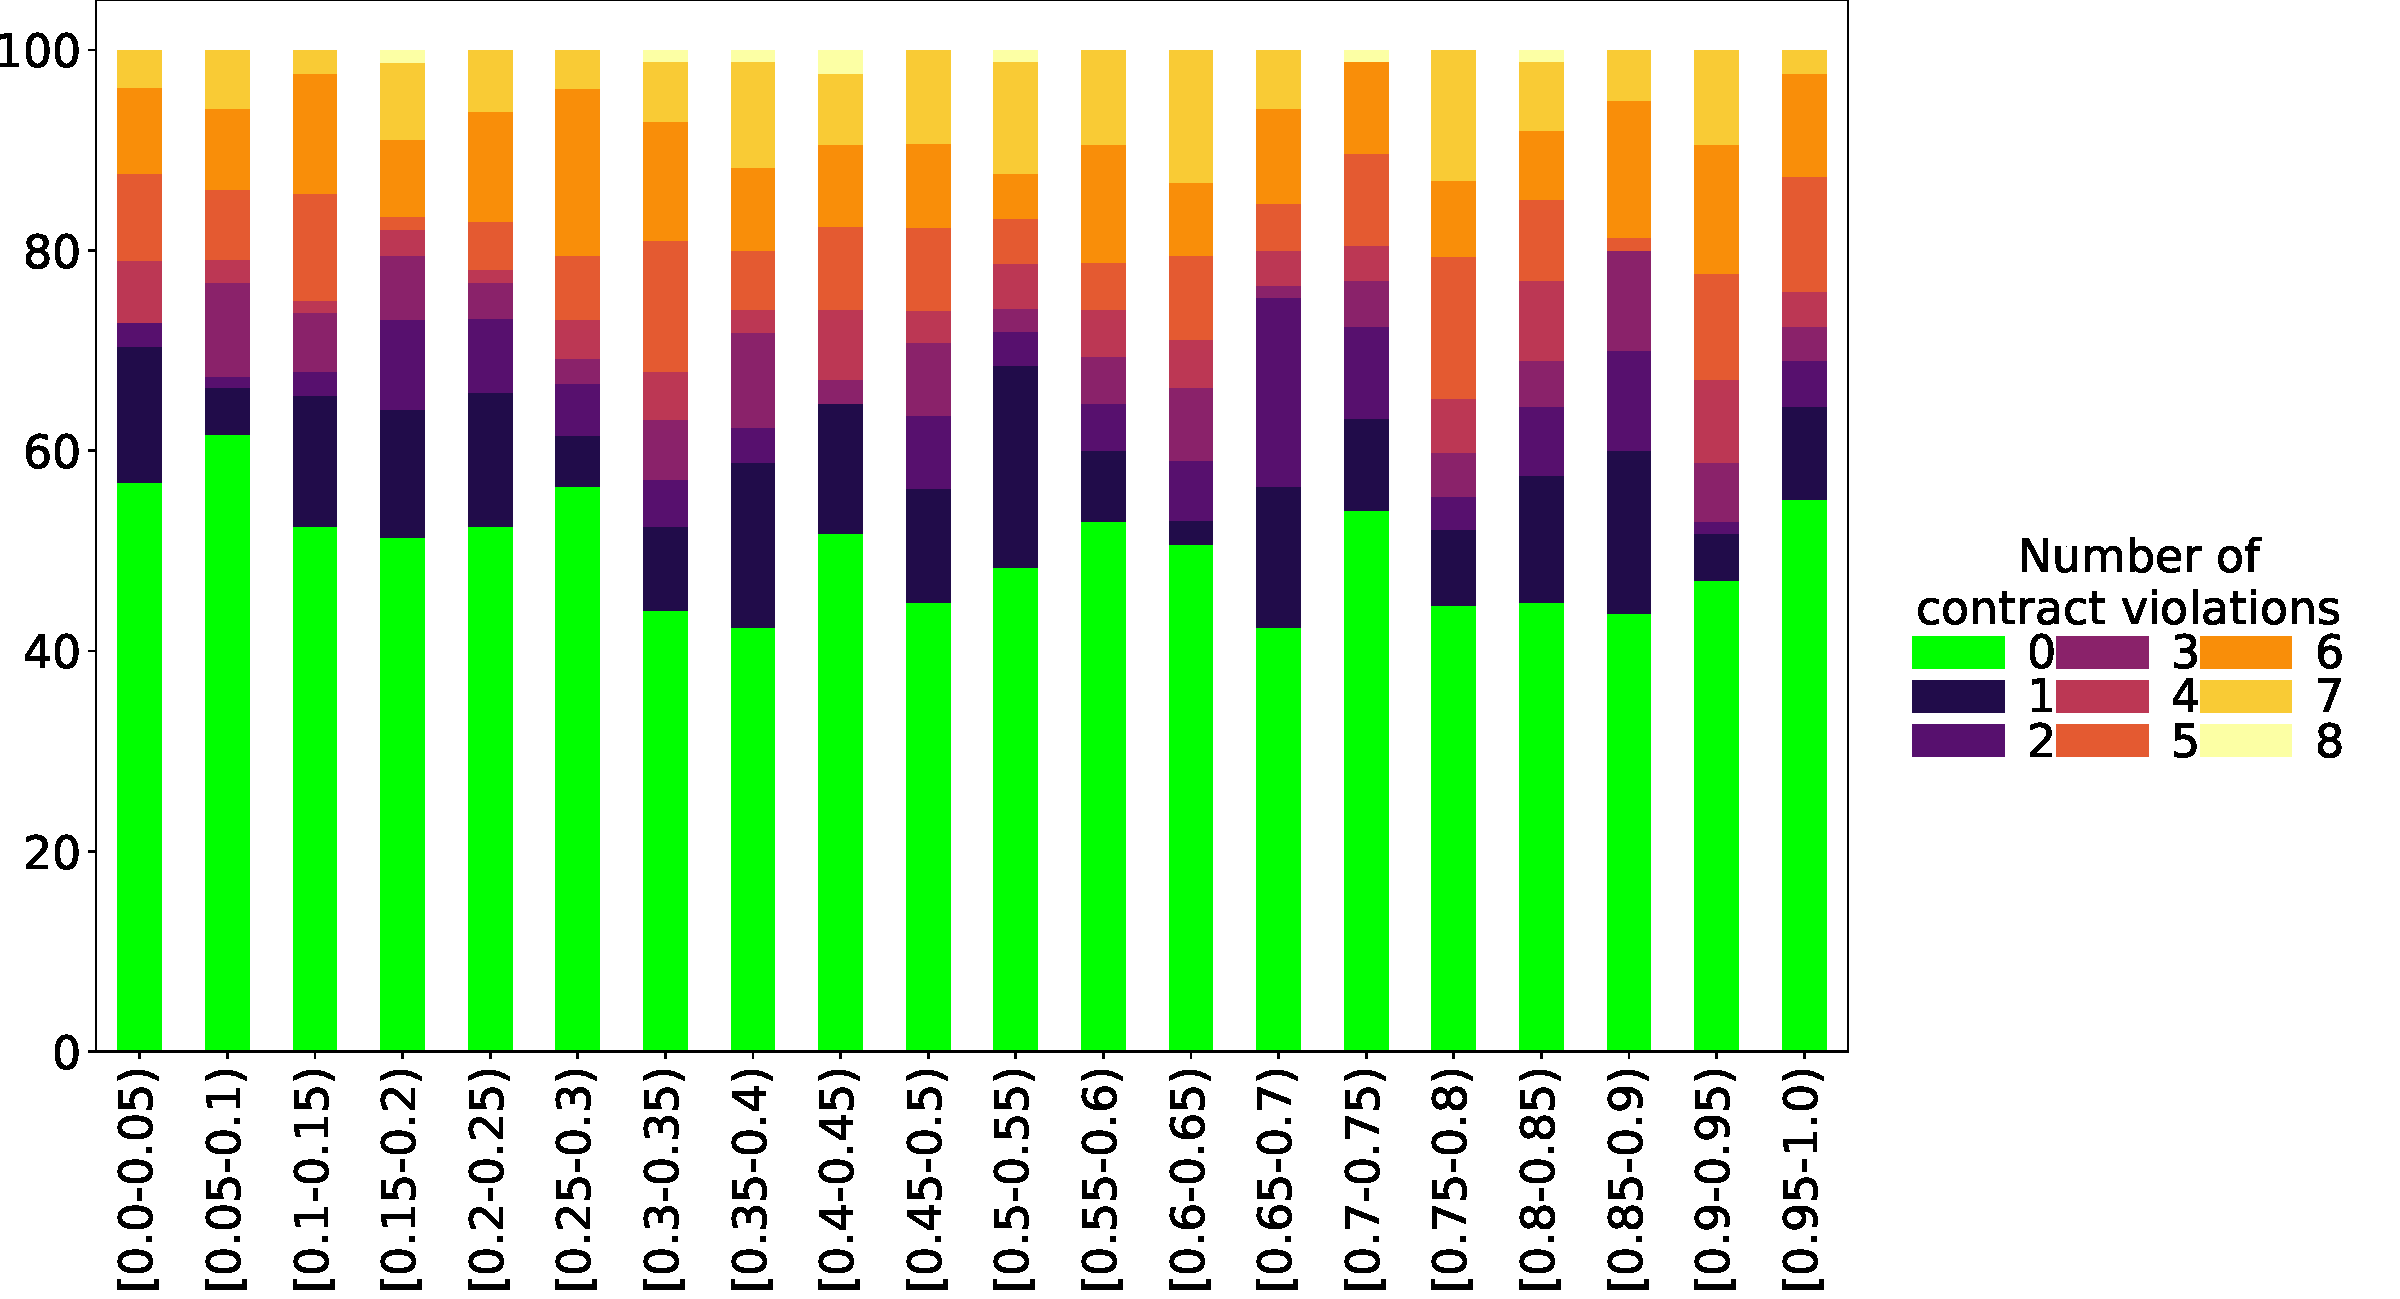
\includegraphics[width=\textwidth]{images/mutationRate_gradient_500dpi.pdf}
	\caption[\texttt{mutationRate}~(R7) parameter values distribution]{\texttt{mutationRate}~(R7) parameter values distribution in terms of contract violations}
	\label{fig:mutationRate_gradient}
\end{figure}

The two types of distribution of parameter values and the number of contract violations are discussed. Distributions for both problems for each parameter presented in Appendix~\ref{appendix:Distributions3}. These plots confirm the conclusions that we made above. Values of some parameters such as \texttt{population\-Size}~(R3), \texttt{crossover\-Rate}~(R5), \texttt{po\-pu\-la\-te\-Soft\-wa\-re\-So\-lu\-tion\-Attempts}~(R13) and \texttt{cross\-over\-On\-Ran\-dom\-Re\-qu\-est\-Pro\-ba\-bi\-li\-ty}~(R16) have a higher influence on the result.
The distribution  of the \texttt{cross\-over\-On\-Ran\-dom\-Re\-quest\-Pro\-ba\-bi\-lity}~(R16) parameter, is showed in Appendix~\ref{appendix:Distributions2}, confirms our conclusions from correlation analysis that lower value gives better result. 
Some parameters give "good" and "bad" results for all values. That means that we could remove them from the parameter tuning and use constant value. Furthermore, for other parameters, values ranges could be adjusted.

\subsection{Parameter Values Distributions in Terms of Quality}
To answer the question of what value of parameters with no obvious advantage in distribution, we construct a similar distribution with the quality of the solution.
In the previous analysis, we presented two distribution for \texttt{populationSize}~(R3) and \texttt{mutationRate}~(R7) parameters for smaller problem for smaller problem.

Figure~\ref{fig:populationSizeObjective} depicts the quality distribution for the \texttt{populationSize}~(R3) parameter. This distribution differs from the previous one shown in Figure~\ref{fig:populationSize_gradientSmall} in terms that all non-valid configurations are located in one segment that marked as "non-valid" and have a black color. Valid results consist of segments with different high and color. Each segment represents the percentage of the total number of configurations that have the same parameter value and which give the result near the same \textbf{quality}. All colors except black show the deviation of the quality of the solution from optimum in percent. \textbf{Green} color represents \textbf{optimal} solutions.

As we can see, if a Genetic Solver gets valid results, the quality of the Solution is optimal, or near-optimal. This distribution also confirms conclusions in Section~\ref{sec:evaluation}.

For current analysis the distribution of the \texttt{mutationRate}~(R7) parameter is more interesting and it is shown in Figure~\ref{fig:mutationRateObjective}. The distribution of contract violations shows that any value of the parameter could give a valid result. However, the distribution of quality shows that some values of the parameter could give an optimal solution to the problem. Let us compare two ranges of values [0.45, 0.5) and [0.75, 0.8). Both ranges have near the same percentage of valid results of 50\%.
Nevertheless, the first range could give an optimal solution. The second range could not give such a solution. Moreover, the percentage of near-optimal solutions for the second range is lower.


\begin{figure}
	\centering
	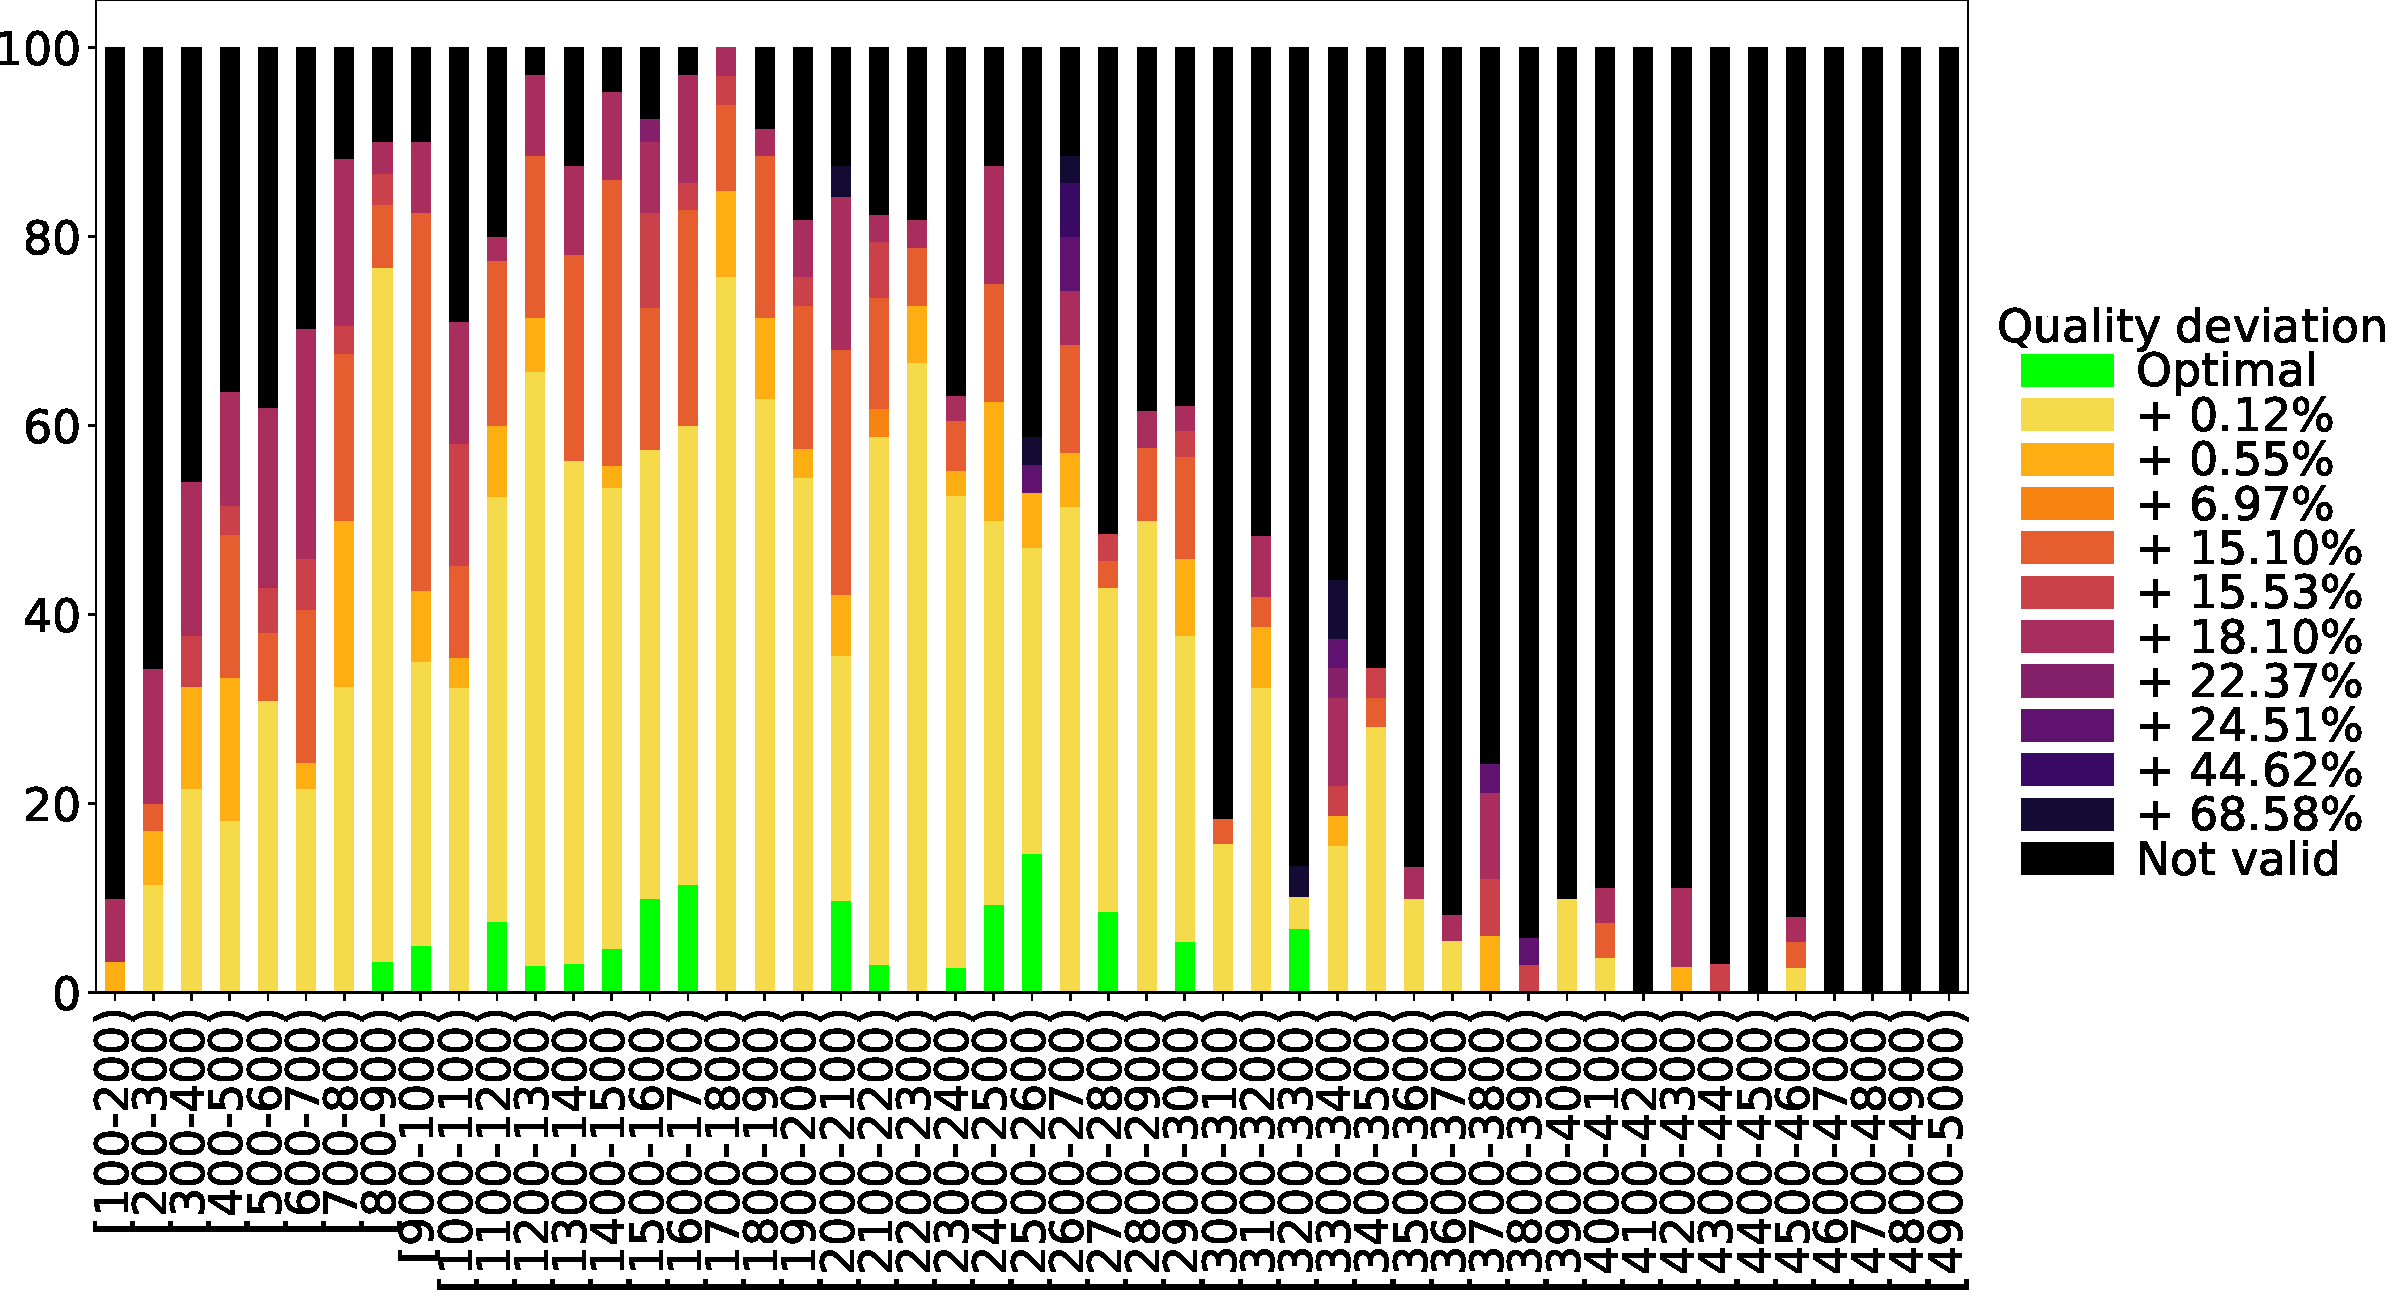
\includegraphics[width=\textwidth]{images/populationSizeObjective.pdf}
	\caption[\texttt{populationSize}~(R3) parameter values distribution in terms of contract violations] {\texttt{populationSize}~(R3) parameter values distribution in terms of quality deviation}
	\label{fig:populationSizeObjective}
\end{figure}


\begin{figure}
	\centering
	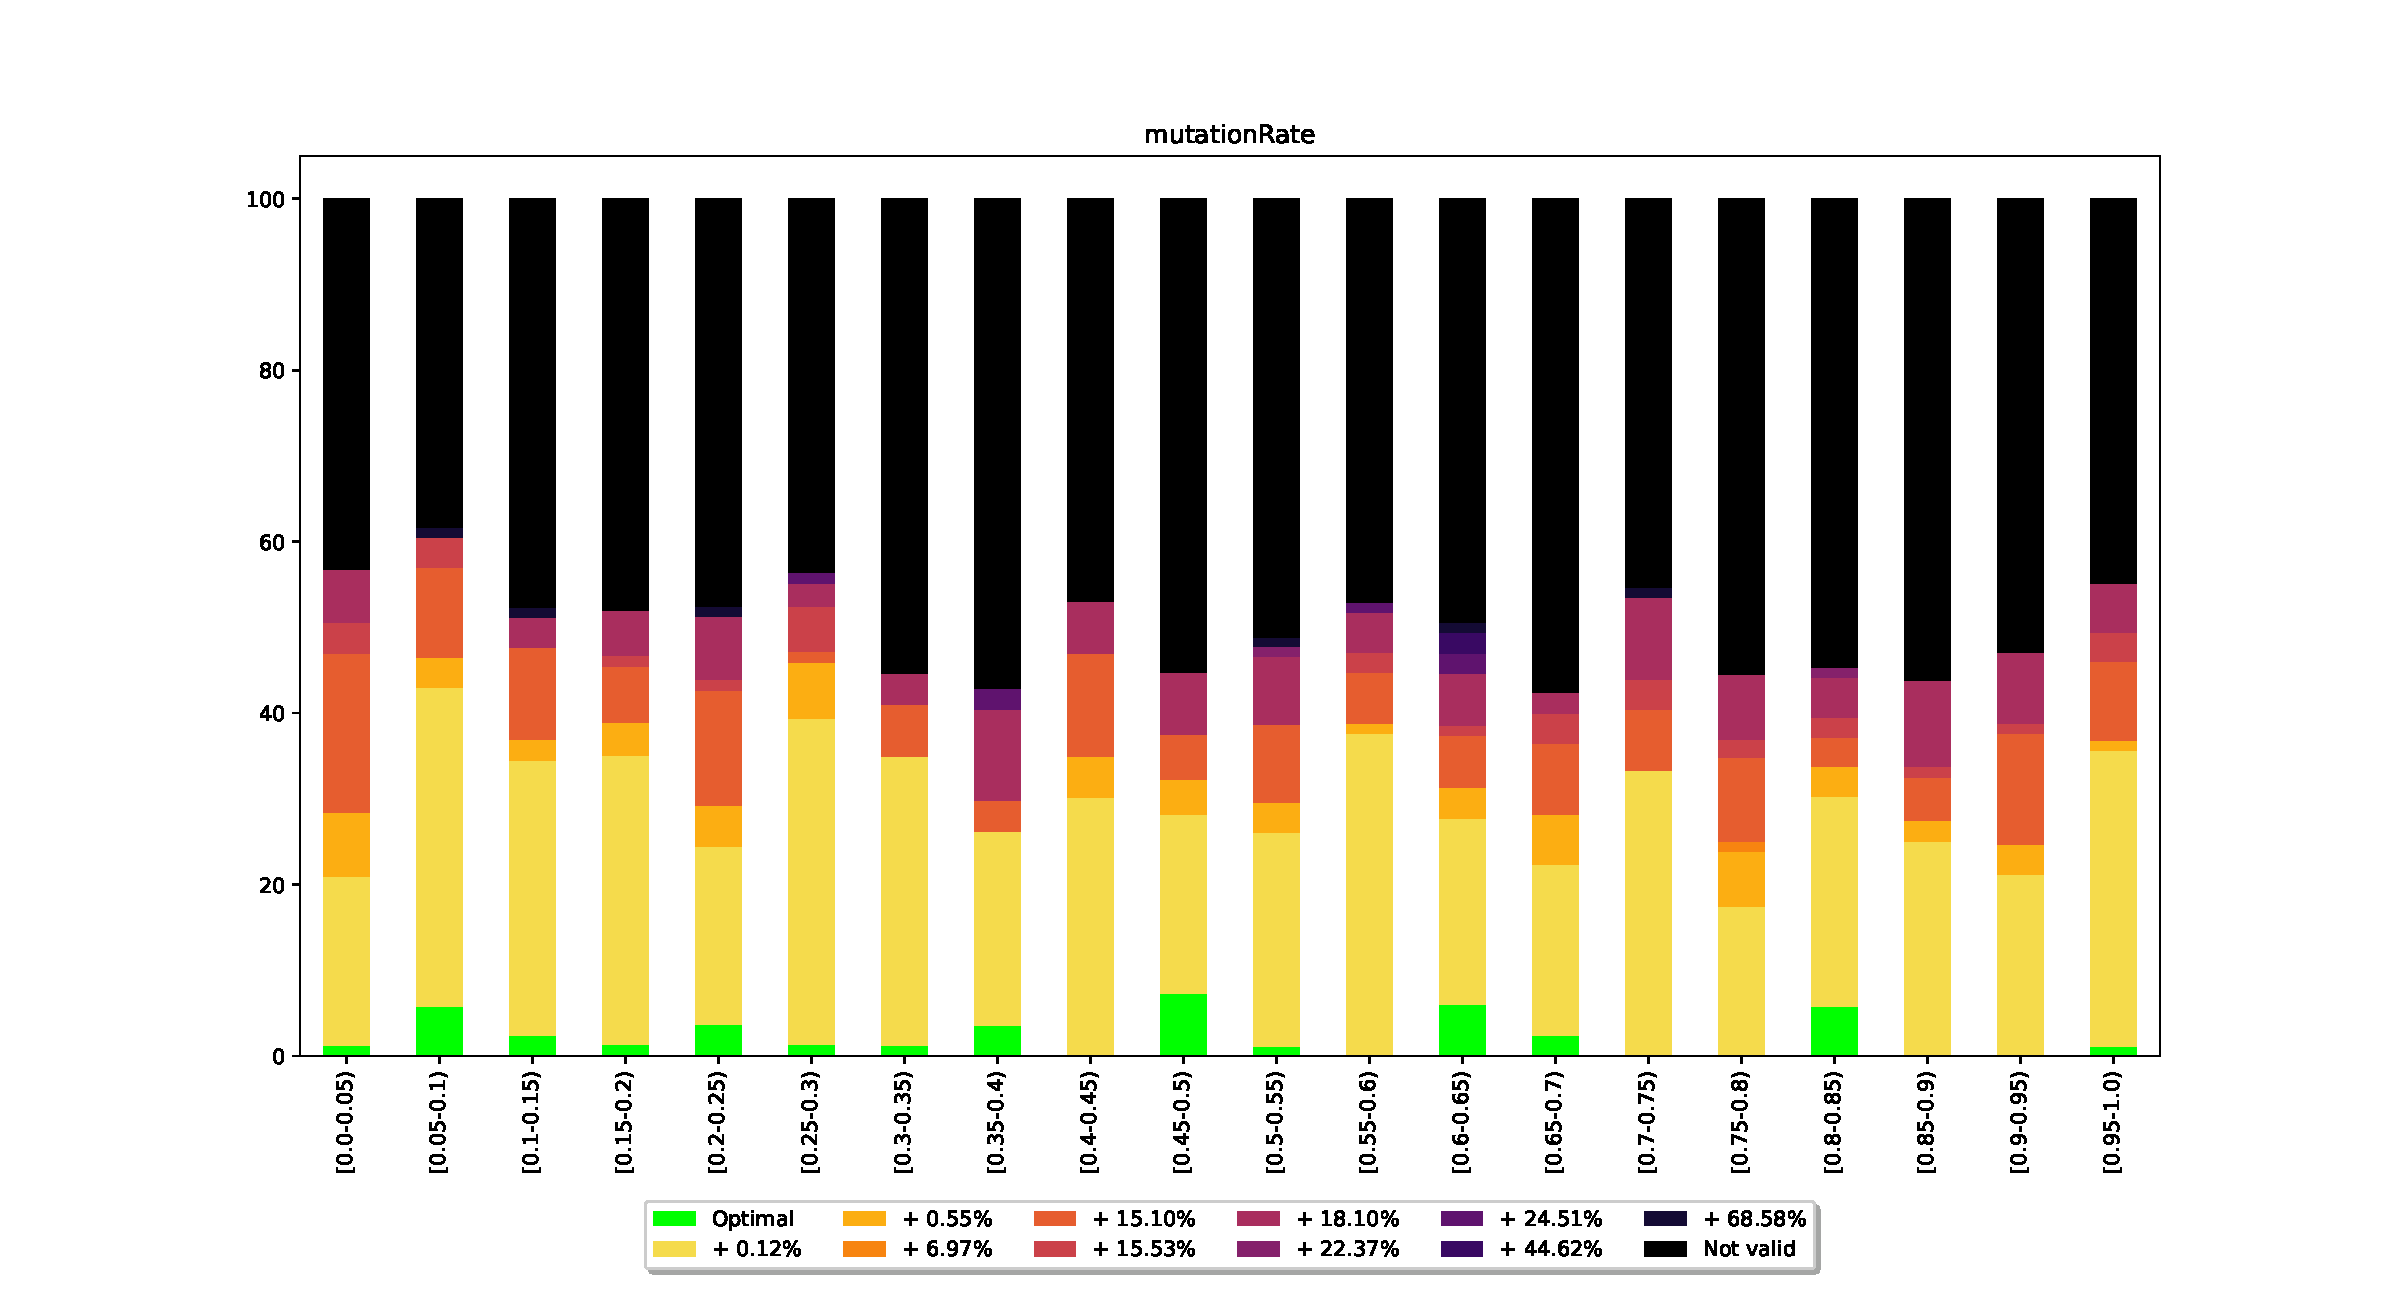
\includegraphics[width=\textwidth]{images/mutationRateObjective.pdf}
	\caption[\texttt{mutationRate}~(R7) parameter values distribution in terms of quality deviation]{\texttt{mutationRate}~(R7) parameter values distribution in terms of quality deviation}
	\label{fig:mutationRateObjective}
\end{figure}

The discussed above plots show that validity of the result in terms of number of contract violations could not depend on the value of the parameter. However, the quality of the solution depends on the parameter value. 

As a conclusion, we could say that we could remove some parameters from the parameter tuning if our goal is to find a valid solution. But we need all parameters if we are looking for the best quality of the solution.